\section*{Приложения}
\addcontentsline{toc}{section}{Приложения}

\counterwithin{figure}{subsection}
\counterwithin{table}{subsection}
\counterwithin{algorithm}{subsection}
\counterwithin{equation}{subsection}

\renewcommand{\thesubsection}{\Alph{subsection}}

\subsection{Алгоритм замены слотов в атаке}

\begin{algorithm}
    \caption{Алгоритм замены слотов в атаке}
    \begin{algorithmic}
        \Function{ExtendSlotLabels}{slot\_label, num\_tokens}
            \\
            \ind slot\_labels = [slot\_label]
            \ind\If{num\_tokens > 1}
                    \ind\ind\If{slot\_label.startswith('B')}
                                \\
                                \ind\ind\ind slot\_labels += ['I' + slot\_label[1:]] $\cdot$ (num\_tokens - 1)
                    \Else
                                \\
                                \ind\ind\ind slot\_labels $\cdot$= num\_tokens
                    \EndIf
            \EndIf \\
            \ind\Return slot\_labels
        \EndFunction
    \end{algorithmic}\label{alg:algorithm3}
\end{algorithm}

\newpage

\subsection{Примеры адверсариальных атак на модели}\label{subsec:examples}

\begin{table}[H]
	\resizebox{\textwidth}{!}{
		\begin{tabular}{|>{\bfseries}l|cccccccccccccc|}
			\hline
			Utterance en &show & me & the & cheapest & one & way & flights & from & montreal & to & orlando &   &   &   \\ \hline
			Utterance adv &spectacle & me & the & Le & moins & cher & one & Le & chemin & vols & de & Montréal & à & Orlando \\ \hline
		\end{tabular}
	}\caption{Пример атаки модели m-BERT (m-bert) word-level атакой.}\label{tab:table24}
\end{table}
\begin{table}[H]
	\resizebox{\textwidth}{!}{
		\begin{tabular}{|>{\bfseries}l|ccccccccc|}
			\hline
			Utterance en &show & me & flights & from & fort & worth & to & san & jose \\ \hline
			Utterance adv &Zeige & me & Flüge & von & fort & worth & nach & San & Jose \\ \hline
		\end{tabular}
	}\caption{Пример атаки модели m-BERT (m-bert) phrase-level атакой.}\label{tab:table25}
\end{table}
\begin{table}[H]
	\resizebox{\textwidth}{!}{
		\begin{tabular}{|>{\bfseries}l|cccccccc|}
			\hline
			Utterance en &find & flight & from & memphis & to & cincinnati & on & sunday \\ \hline
			Utterance adv &Encontrar & flight & from & Memphis & to & cincinnati & En & sunday \\ \hline
		\end{tabular}
	}\caption{Пример атаки модели m-BERT (m-bert en) word-level атакой.}\label{tab:table26}
\end{table}
\begin{table}[H]
	\resizebox{\textwidth}{!}{
		\begin{tabular}{|>{\bfseries}l|cccccccc|}
			\hline
			Utterance en &please & list & flights & from & philadelphia & to & san & francisco \\ \hline
			Utterance adv &bitte & bitte & flights & from & Philadelphia & to & San & Francisco \\ \hline
		\end{tabular}
	}\caption{Пример атаки модели m-BERT (m-bert en) phrase-level атакой.}\label{tab:table27}
\end{table}
\begin{table}[H]
	\resizebox{\textwidth}{!}{
		\begin{tabular}{|>{\bfseries}l|ccccccccccc|}
			\hline
			Utterance en &list & a & flight & on & american & airlines & from & toronto & to & san & diego \\ \hline
			Utterance adv &Lista & a & flight & on & estadounidense & Aerolíneas & de & Torrente & to & San & Diego \\ \hline
		\end{tabular}
	}\caption{Пример атаки модели m-BERT (m-bert adv) word-level атакой.}\label{tab:table28}
\end{table}
\begin{table}[H]
	\resizebox{\textwidth}{!}{
		\begin{tabular}{|>{\bfseries}l|ccccccccc|}
			\hline
			Utterance en &show & me & all & the & flights & from & burbank & to & milwaukee \\ \hline
			Utterance adv &show & me & todos & the & voos & from & Burbank & to & Milwaukee \\ \hline
		\end{tabular}
	}\caption{Пример атаки модели m-BERT (m-bert adv) phrase-level атакой.}\label{tab:table29}
\end{table}
\begin{table}[H]
	\resizebox{\textwidth}{!}{
		\begin{tabular}{|>{\bfseries}l|ccccccccccc|}
			\hline
			Utterance en &what & flights & travel & from & las & vegas & to & los & angeles &   &   \\ \hline
			Utterance adv &Ce & que & vols & travel & de & Les & VEGAS & to & los & Les & Anges \\ \hline
		\end{tabular}
	}\caption{Пример атаки модели m-BERT (m-bert en + adv) word-level атакой.}\label{tab:table30}
\end{table}
\begin{table}[H]
	\resizebox{\textwidth}{!}{
		\begin{tabular}{|>{\bfseries}l|cccccccccccccc|}
			\hline
			Utterance en &list & american & airlines & flights & from & houston & to & milwaukee & departing & friday & pm &   &   &   \\ \hline
			Utterance adv &list & American & Airlines & -Flüge & flights & from & Houston & nach & Milwaukee & abfliegen & die & Freitag & nachmittag & pm \\ \hline
		\end{tabular}
	}\caption{Пример атаки модели m-BERT (m-bert en + adv) phrase-level атакой.}\label{tab:table31}
\end{table}

\begin{table}[H]
	\resizebox{\textwidth}{!}{
		\begin{tabular}{|>{\bfseries}l|cccccccccc|}
			\hline
			Utterance en &please & list & the & flights & from & newark & to & los & angeles &   \\ \hline
			Utterance adv &please & Liste & Le & flights & de & newark & to & los & Les & Anges \\ \hline
		\end{tabular}
	}\caption{Пример атаки модели XLM-RoBERTa (xlm-r) word-level атакой.}\label{tab:table32}
\end{table}
\begin{table}[H]
	\resizebox{\textwidth}{!}{
		\begin{tabular}{|>{\bfseries}l|cccccccccc|}
			\hline
			Utterance en &show & me & the & nonstop & flights & from & toronto & to & st. & petersburg \\ \hline
			Utterance adv &show & me & the & nonstop & vuelos & de & toronto & a & san & petersburg \\ \hline
		\end{tabular}
	}\caption{Пример атаки модели XLM-RoBERTa (xlm-r) phrase-level атакой.}\label{tab:table33}
\end{table}
\begin{table}[H]
	\resizebox{\textwidth}{!}{
		\begin{tabular}{|>{\bfseries}l|ccccccccccccc|}
			\hline
			Utterance en &list & flights & from & seattle & to & salt & lake & city & on & delta & be1 &   &   \\ \hline
			Utterance adv &list & flights & from & Seattle & to & salt & El & lago & city & En & El & delta & B1 \\ \hline
		\end{tabular}
	}\caption{Пример атаки модели XLM-RoBERTa (xlm-r en) word-level атакой.}\label{tab:table34}
\end{table}
\begin{table}[H]
	\resizebox{\textwidth}{!}{
		\begin{tabular}{|>{\bfseries}l|ccccccccccc|}
			\hline
			Utterance en &which & different & airlines & go & from & las & vegas & to & new & york & city \\ \hline
			Utterance adv &which & different & aériennes & go & from & Las & vegas & à & New & York & City \\ \hline
		\end{tabular}
	}\caption{Пример атаки модели XLM-RoBERTa (xlm-r en) phrase-level атакой.}\label{tab:table35}
\end{table}
\begin{table}[H]
	\resizebox{\textwidth}{!}{
		\begin{tabular}{|>{\bfseries}l|ccccccccccccc|}
			\hline
			Utterance en &list & the & flights & from & westchester & county & to & denver & on & june & seventh &   &   \\ \hline
			Utterance adv &Lista & the & vuelos & from & El & Westchester & Condado & para & El & Denver & on & Junio & seventh \\ \hline
		\end{tabular}
	}\caption{Пример атаки модели XLM-RoBERTa (xlm-r adv) word-level атакой.}\label{tab:table36}
\end{table}
\begin{table}[H]
	\resizebox{\textwidth}{!}{
		\begin{tabular}{|>{\bfseries}l|cccccccccc|}
			\hline
			Utterance en &which & flights & on & us & air & go & from & orlando & to & cleveland \\ \hline
			Utterance adv &Quels & vols & d’ & US & Air & go & d’ & orlando & to & cleveland \\ \hline
		\end{tabular}
	}\caption{Пример атаки модели XLM-RoBERTa (xlm-r adv) phrase-level атакой.}\label{tab:table37}
\end{table}
\begin{table}[H]
	\resizebox{\textwidth}{!}{
		\begin{tabular}{|>{\bfseries}l|ccccccccc|}
			\hline
			Utterance en &show & me & the & flights & between & houston & and & orlando &   \\ \hline
			Utterance adv &spectacle & me & Le & vols & between & à & Houston & et & Orlando \\ \hline
		\end{tabular}
	}\caption{Пример атаки модели XLM-RoBERTa (xlm-r en + adv) word-level атакой.}\label{tab:table38}
\end{table}
\begin{table}[H]
	\resizebox{\textwidth}{!}{
		\begin{tabular}{|>{\bfseries}l|cccccccc|}
			\hline
			Utterance en &show & me & the & flights & between & houston & and & orlando \\ \hline
			Utterance adv &muéstrame & muéstrame & los & vuelos & between & houston & y & orlando \\ \hline
		\end{tabular}
	}\caption{Пример атаки модели XLM-RoBERTa (xlm-r en + adv) phrase-level атакой.}\label{tab:table39}
\end{table}


\newpage

\subsection{Графики с результатами экспериментов}\label{subsec:graphs}

\begin{figure}[H]
    \centering
    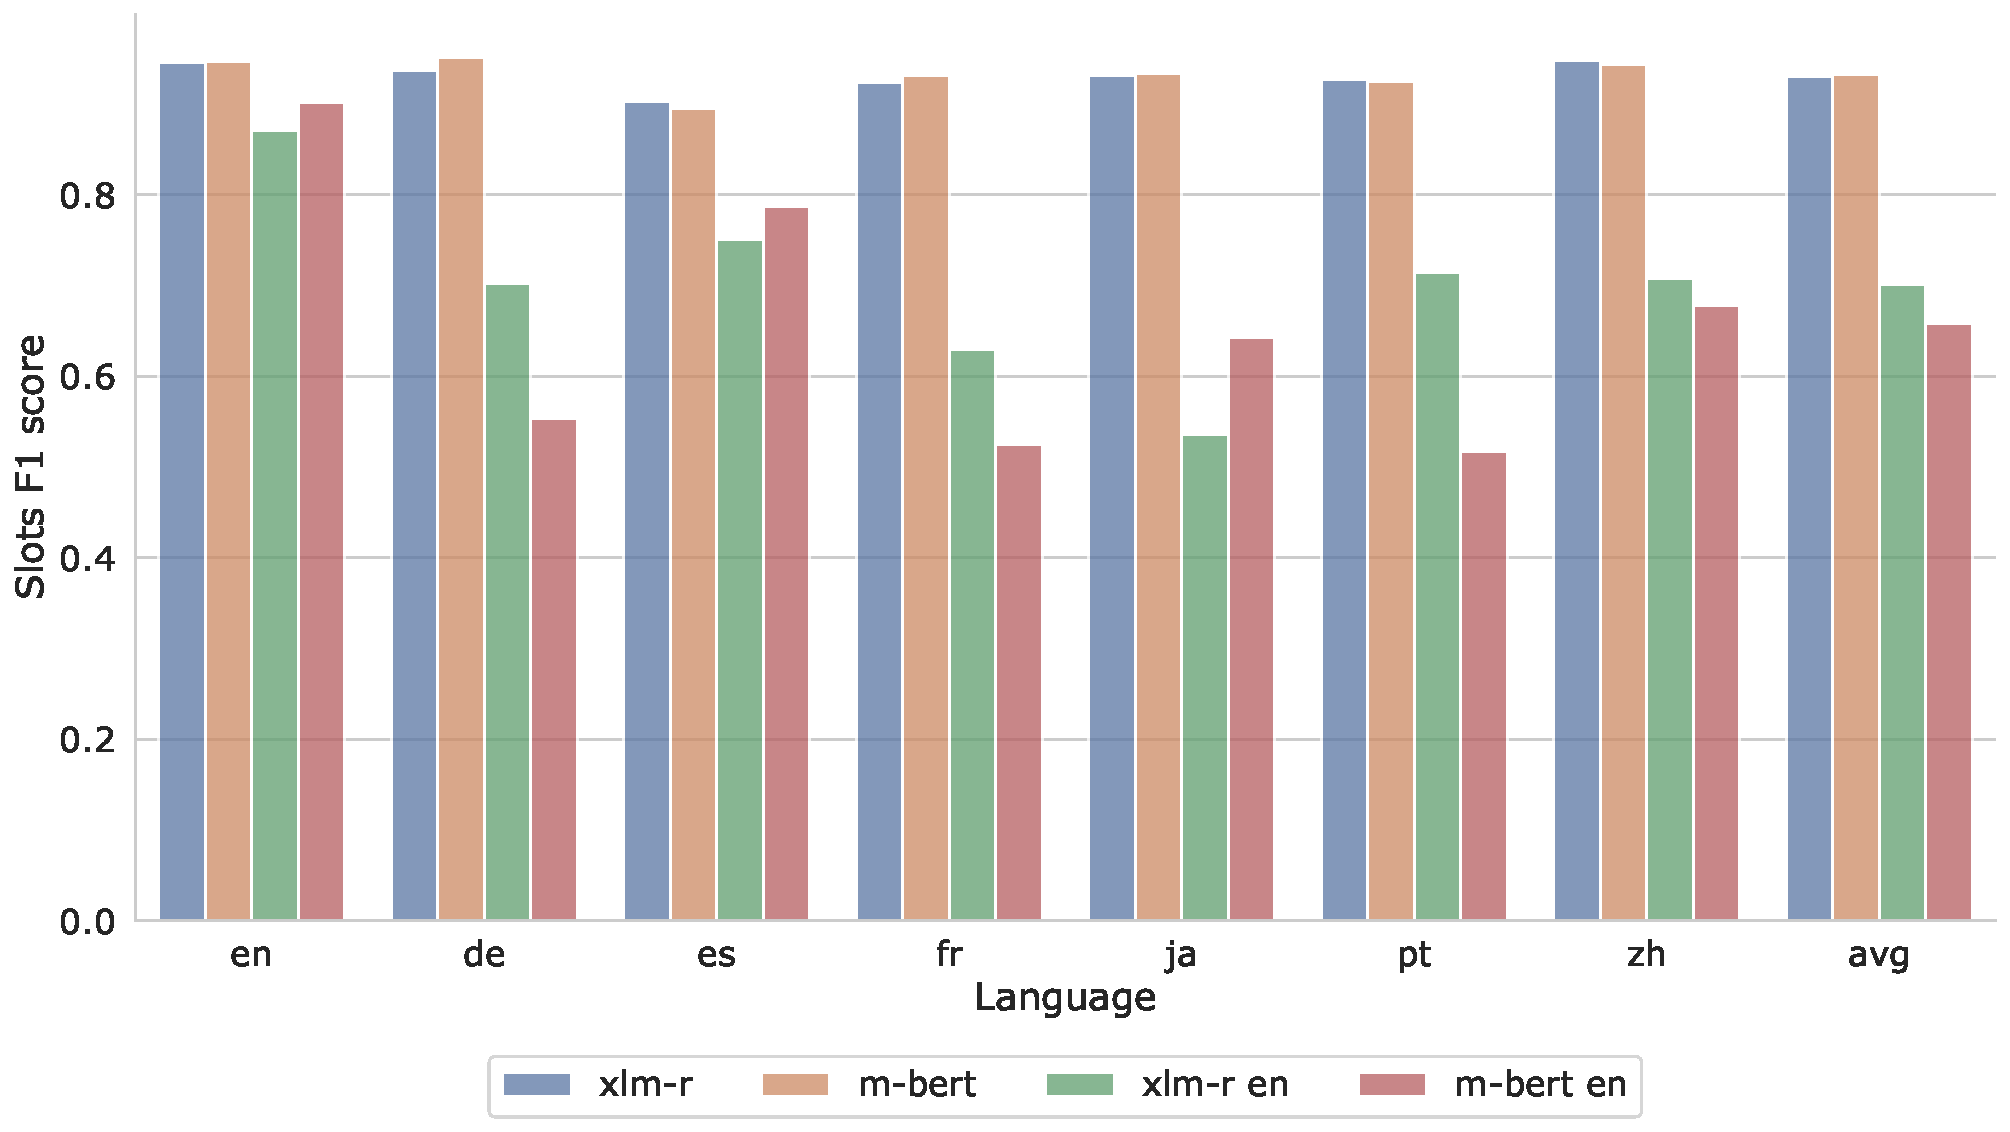
\includegraphics[width=\textwidth]{images/1}
    \caption{Сравнение моделей между собой \textbf{на тестовой выборке} датасета MultiAtis++ по метрике \textbf{Slots F1 score}.}\label{fig:figure1}
\end{figure}
\begin{figure}[H]
    \centering
    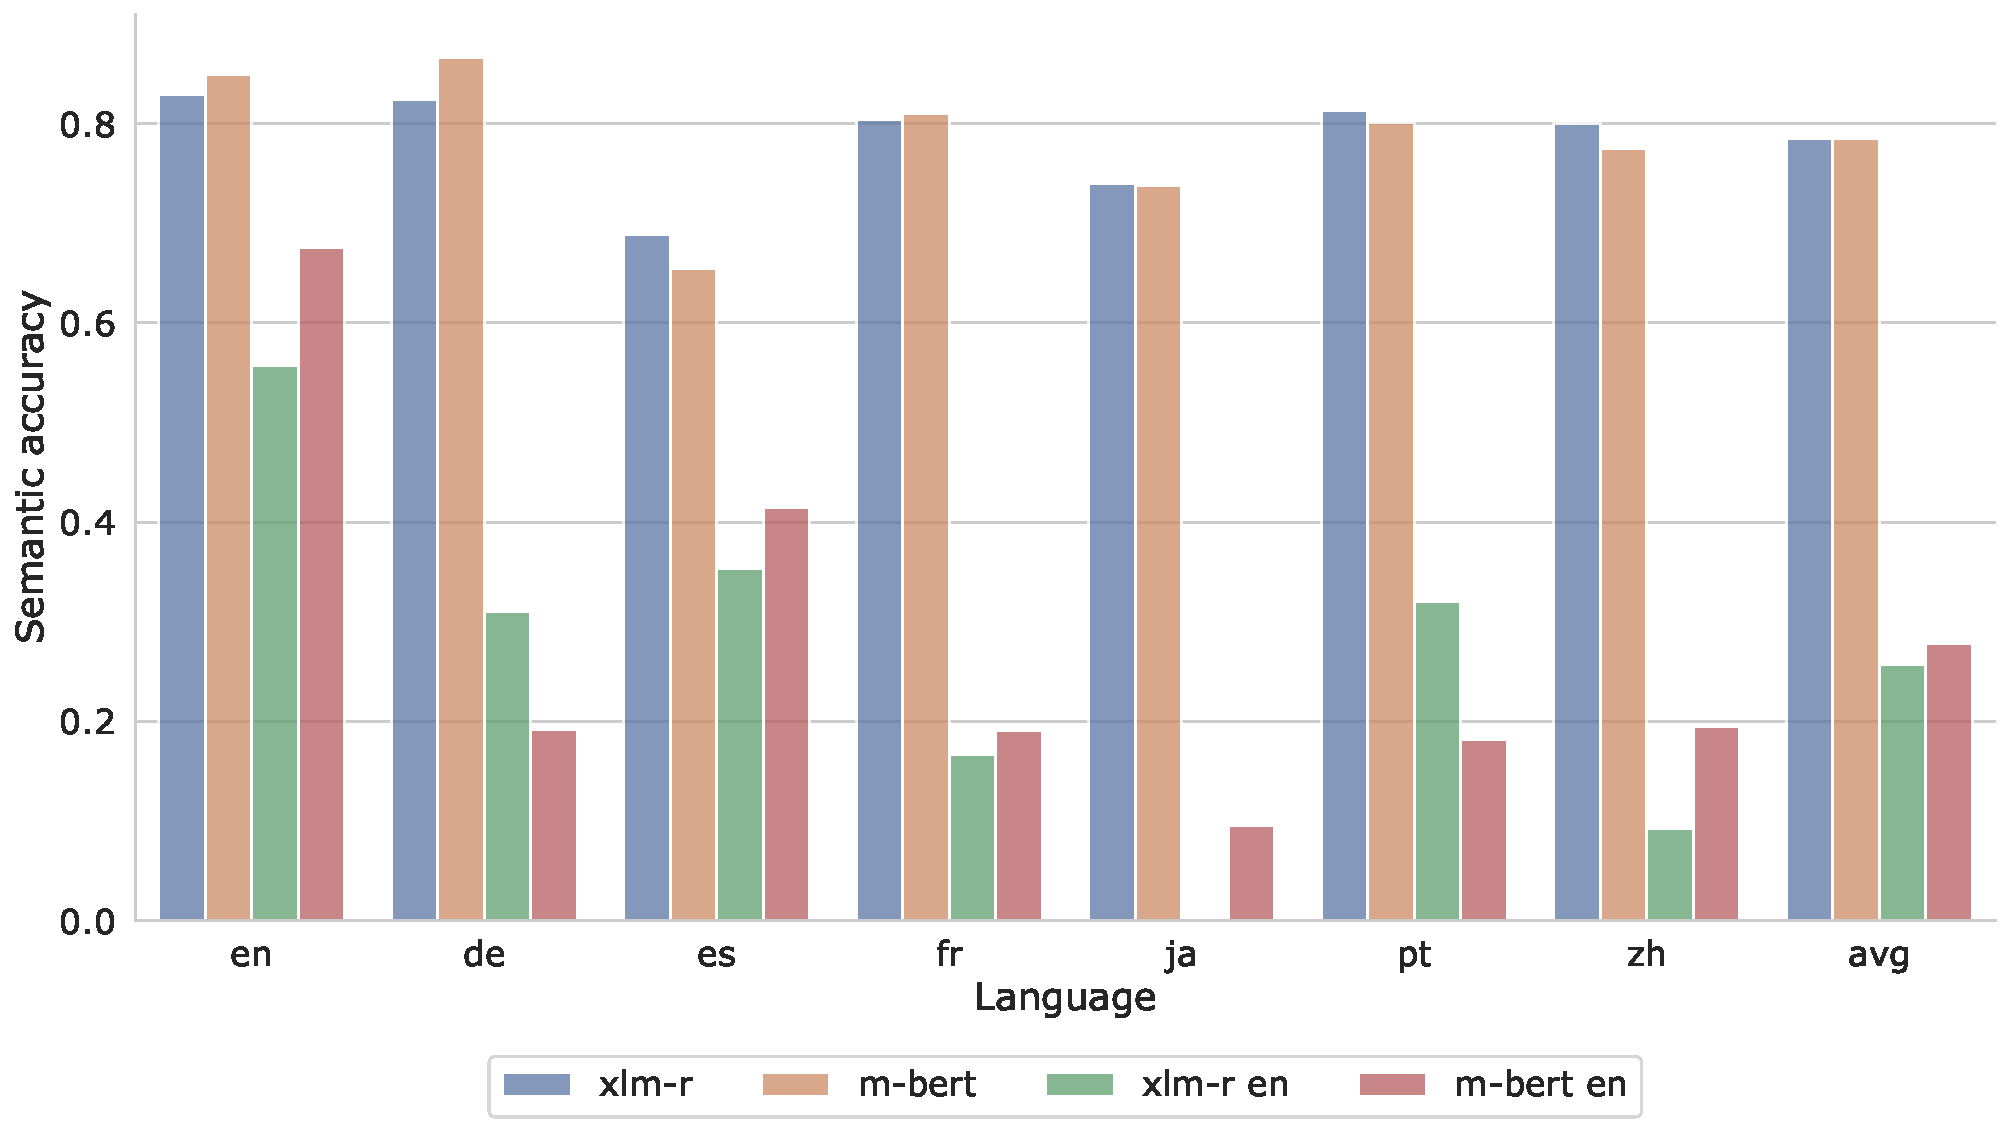
\includegraphics[width=\textwidth]{images/2}
    \caption{Сравнение моделей между собой \textbf{на тестовой выборке} датасета MultiAtis++ по метрике \textbf{Semantic accuracy}.}\label{fig:figure2}
\end{figure}

\begin{figure}[H]
    \centering
    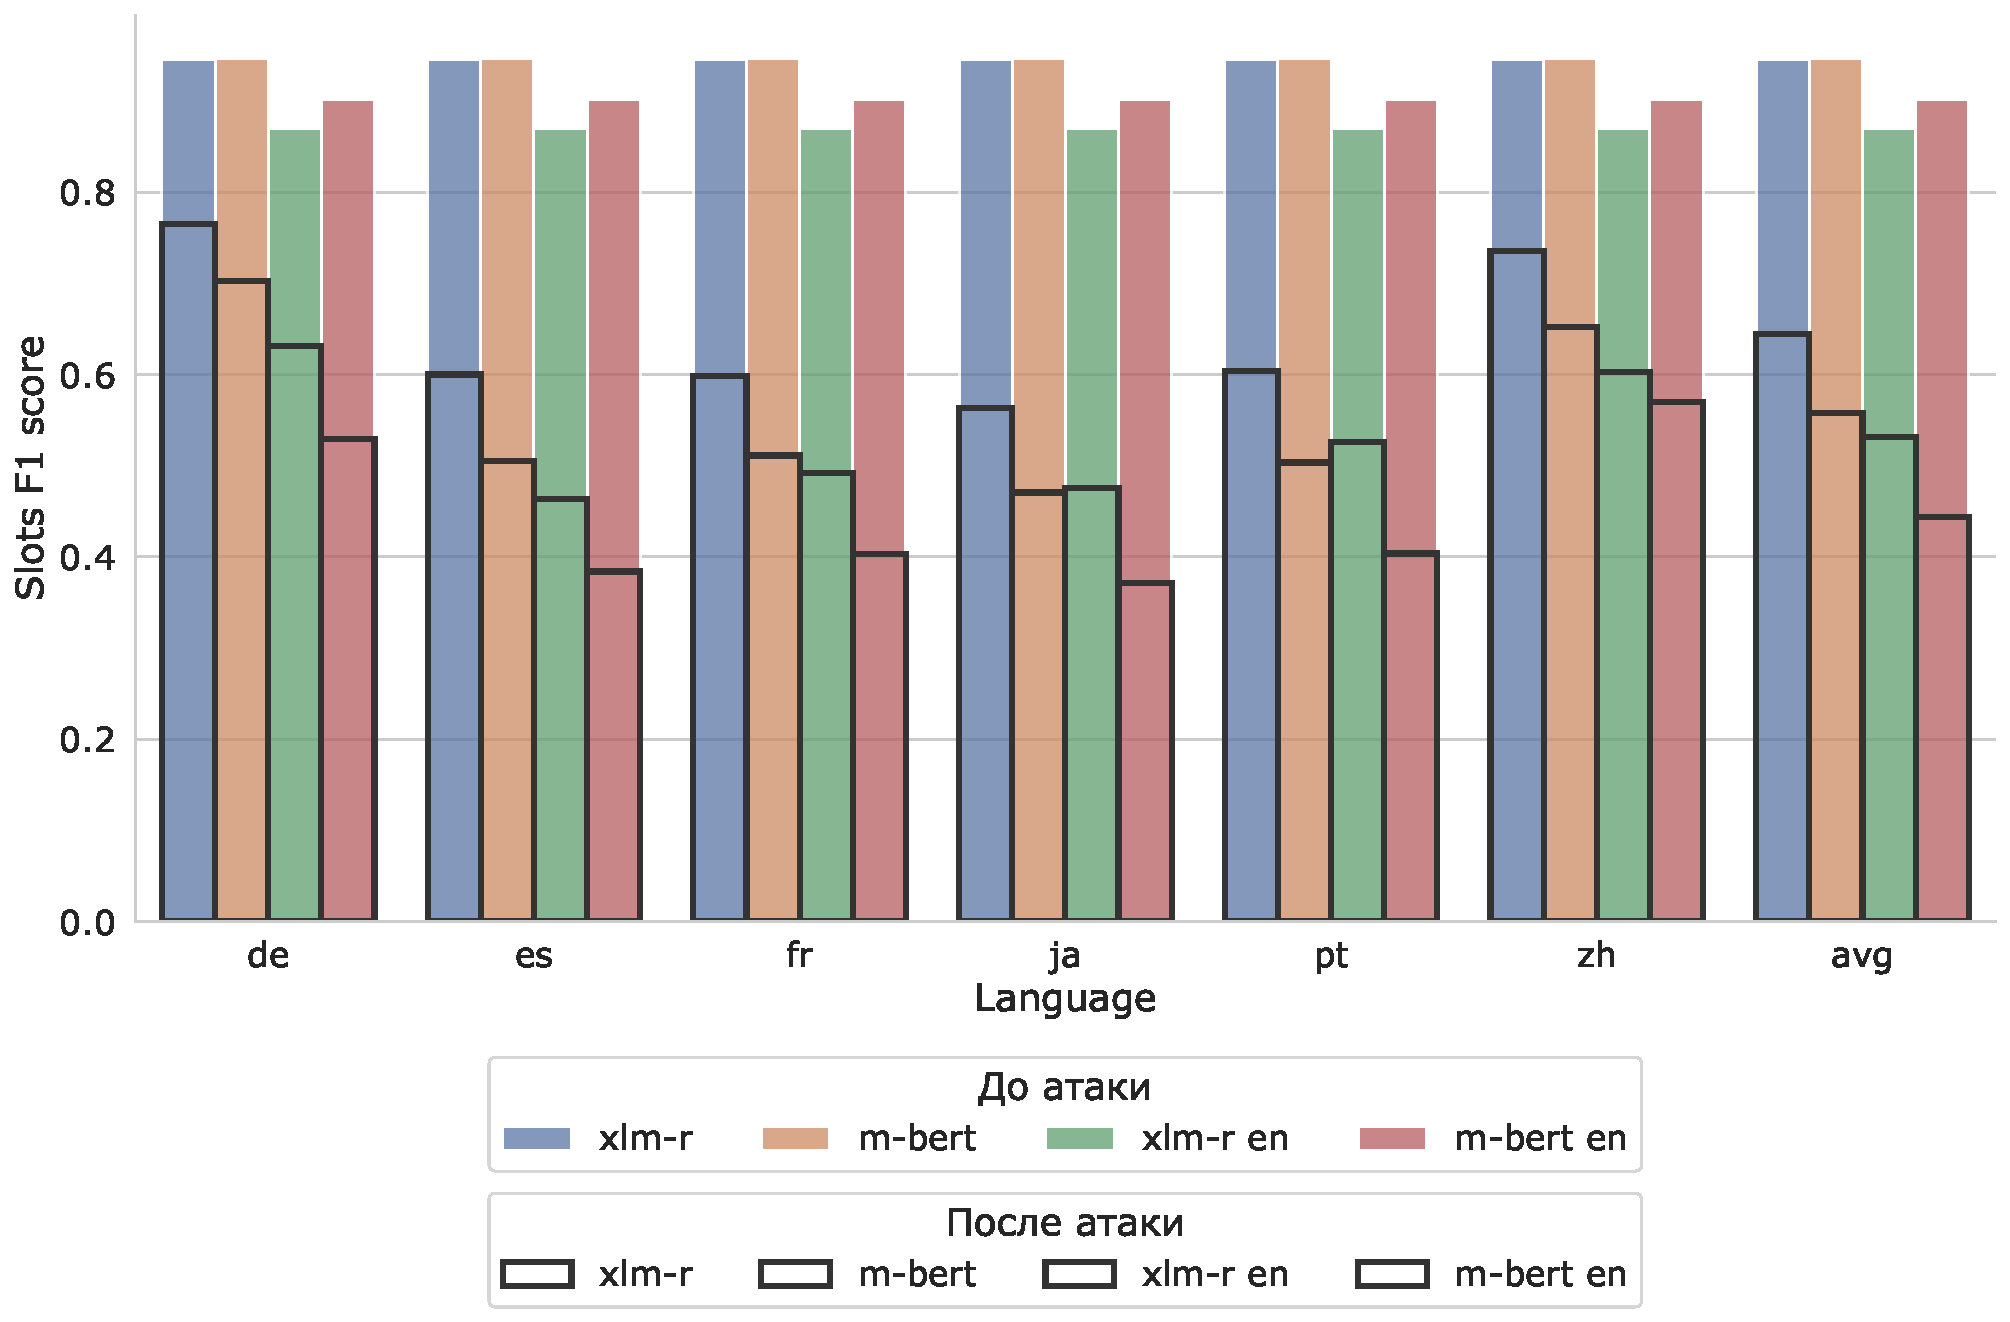
\includegraphics[width=\textwidth]{images/4}
    \caption{Сравнение моделей между собой после \textbf{word-level} атаки на тестовую выборку датасета MultiAtis++ по метрике \textbf{Slots F1 score}.}\label{fig:figure4}
\end{figure}
\begin{figure}[H]
    \centering
    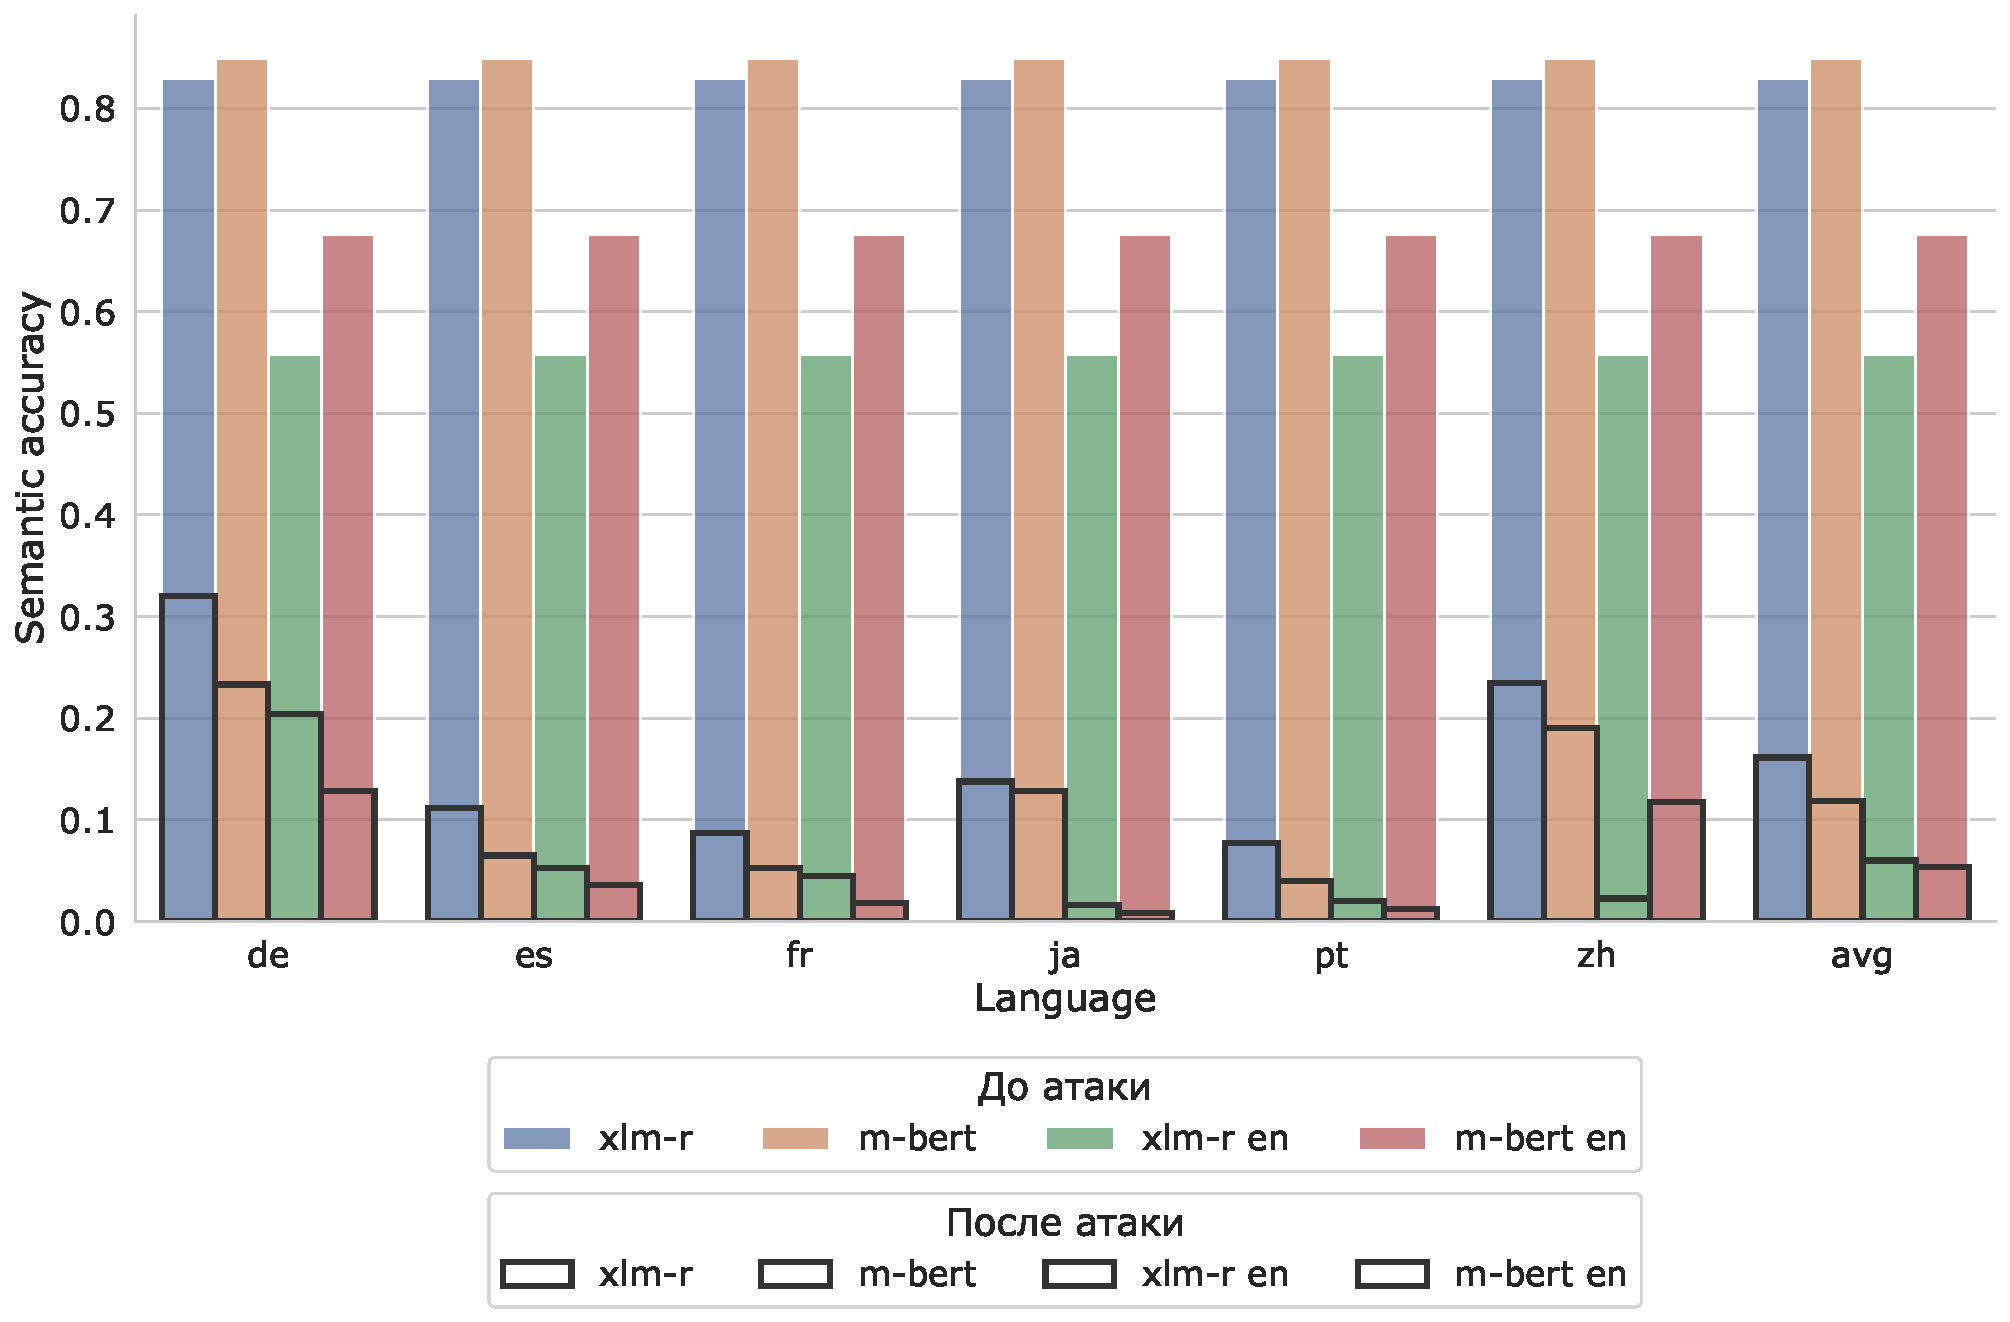
\includegraphics[width=\textwidth]{images/5}
    \caption{Сравнение моделей между собой после \textbf{word-level} атаки на тестовую выборку датасета MultiAtis++ по метрике \textbf{Semantic accuracy}.}\label{fig:figure5}
\end{figure}

\begin{figure}[H]
    \centering
    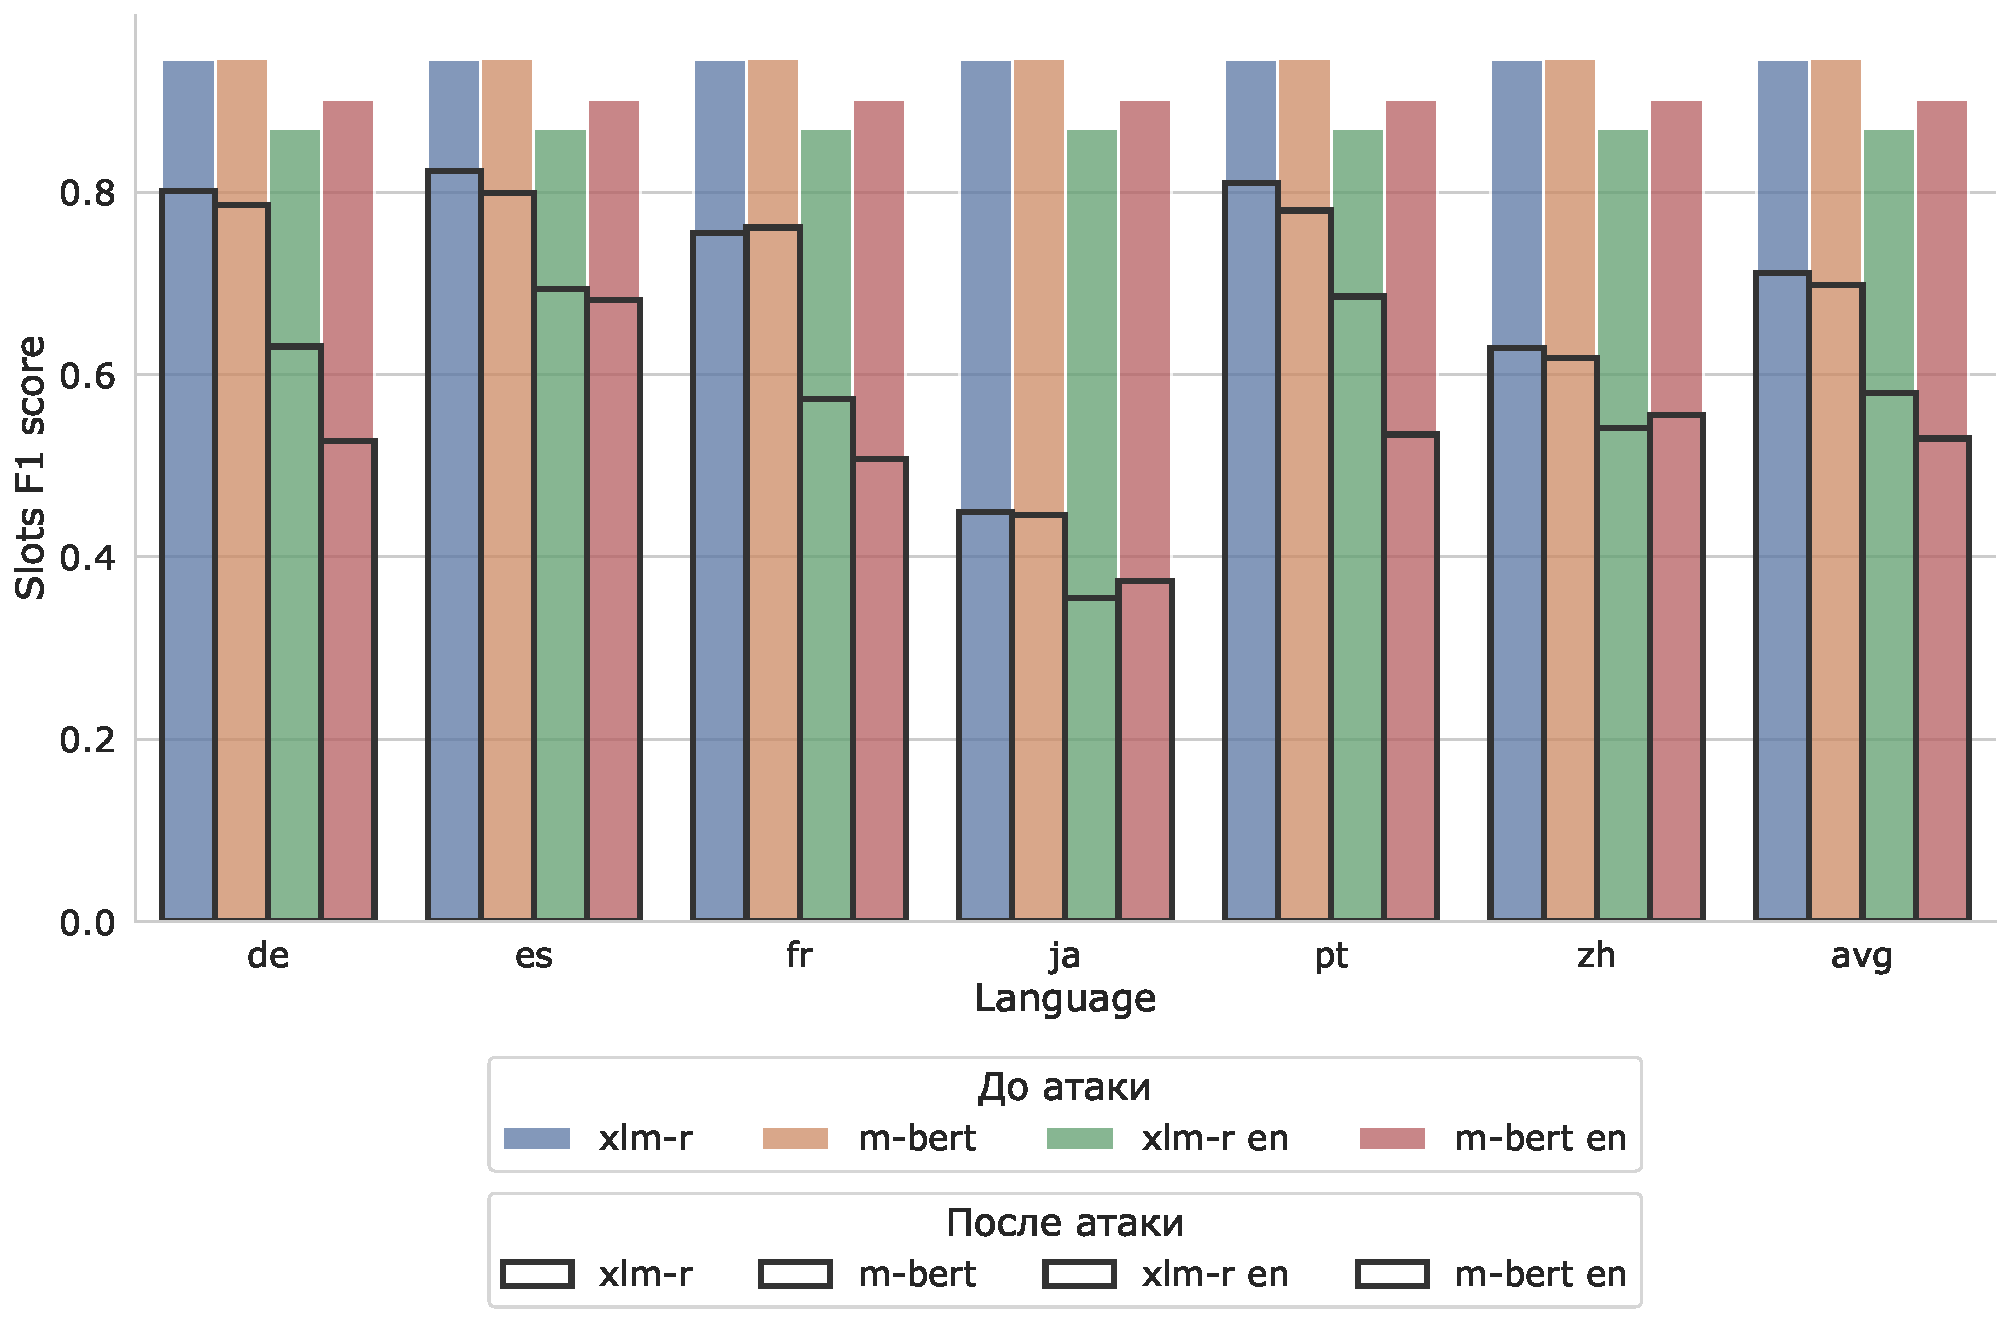
\includegraphics[width=\textwidth]{images/7}
    \caption{Сравнение моделей между собой после \textbf{phrase-level} атаки на тестовую выборку датасета MultiAtis++ по метрике \textbf{Slots F1 score}.}\label{fig:figure7}
\end{figure}
\begin{figure}[H]
    \centering
    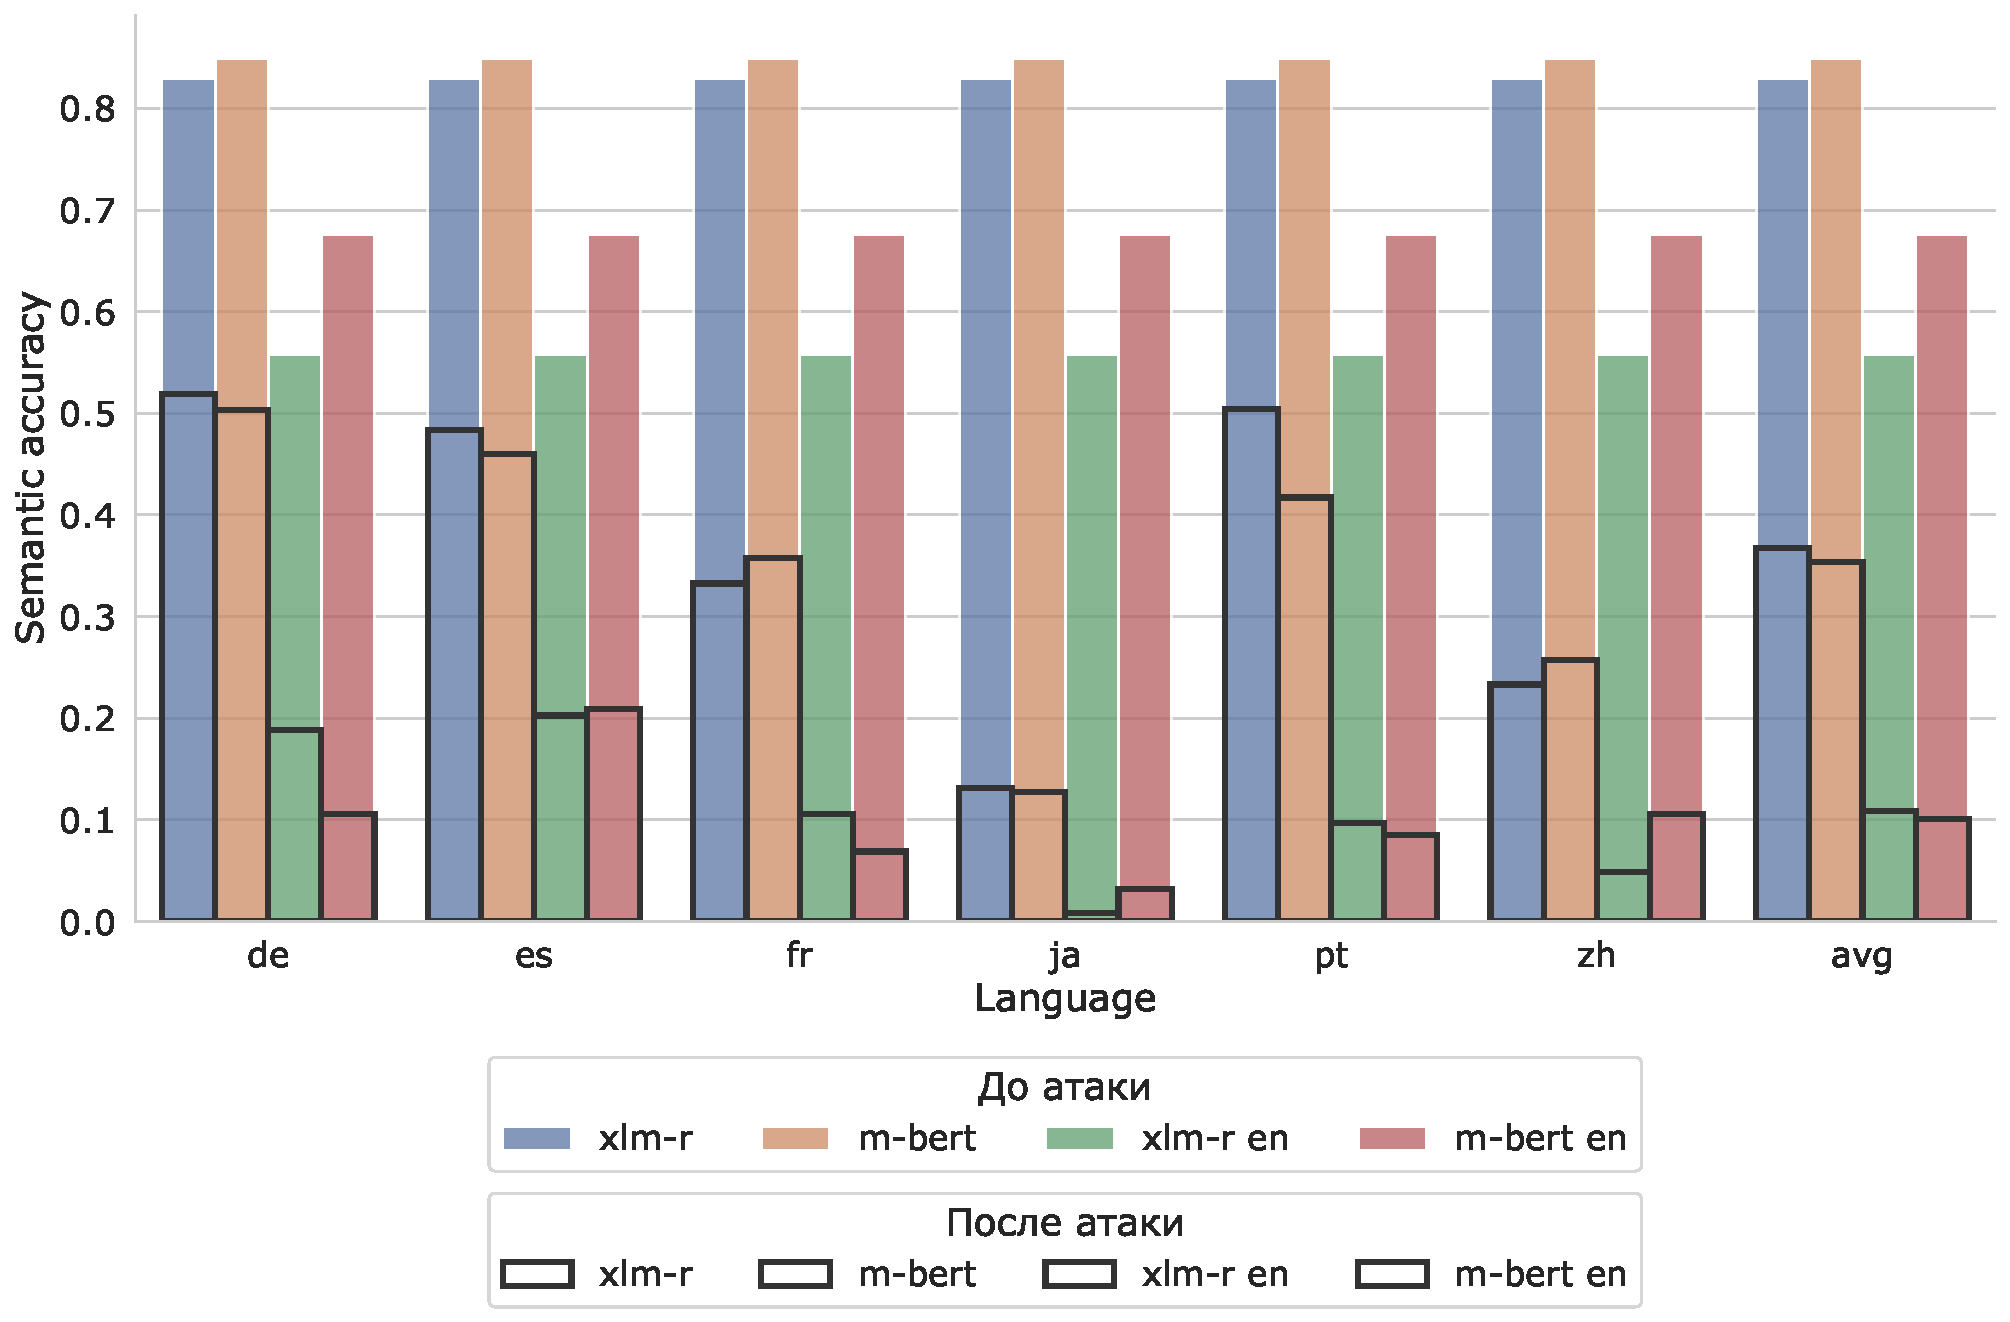
\includegraphics[width=\textwidth]{images/8}
    \caption{Сравнение моделей между собой после \textbf{phrase-level} атаки на тестовую выборку датасета MultiAtis++ по метрике \textbf{Semantic accuracy}.}\label{fig:figure8}
\end{figure}

\begin{figure}[H]
    \centering
    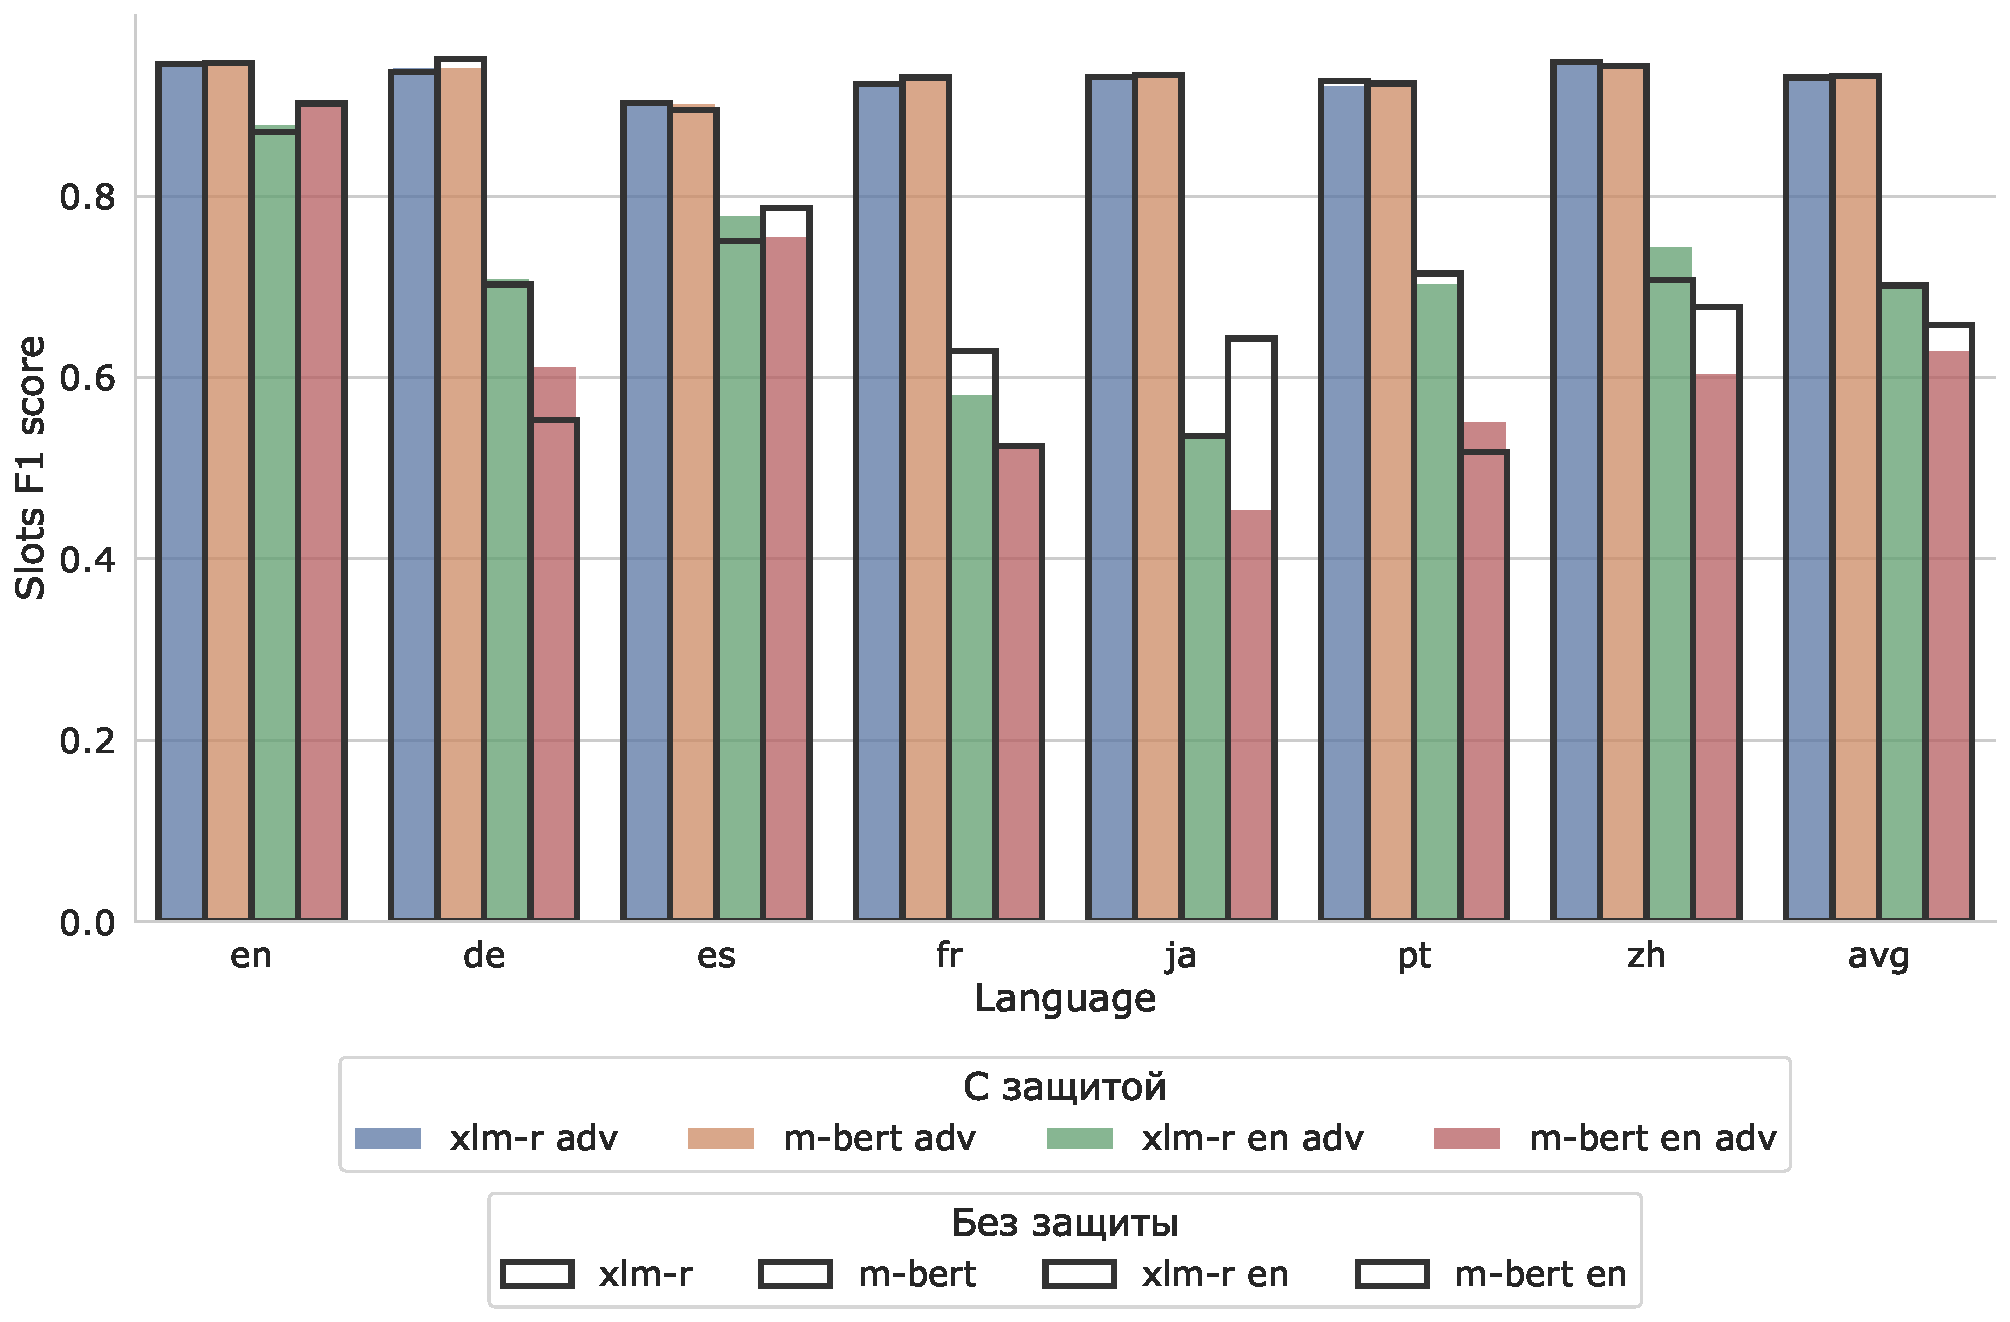
\includegraphics[width=\textwidth]{images/10}
    \caption{Сравнение моделей \textbf{с защитой} между собой \textbf{на тестовой выборке} датасета MultiAtis++ по метрике \textbf{Slots F1 score}.}\label{fig:figure10}
\end{figure}
\begin{figure}[H]
    \centering
    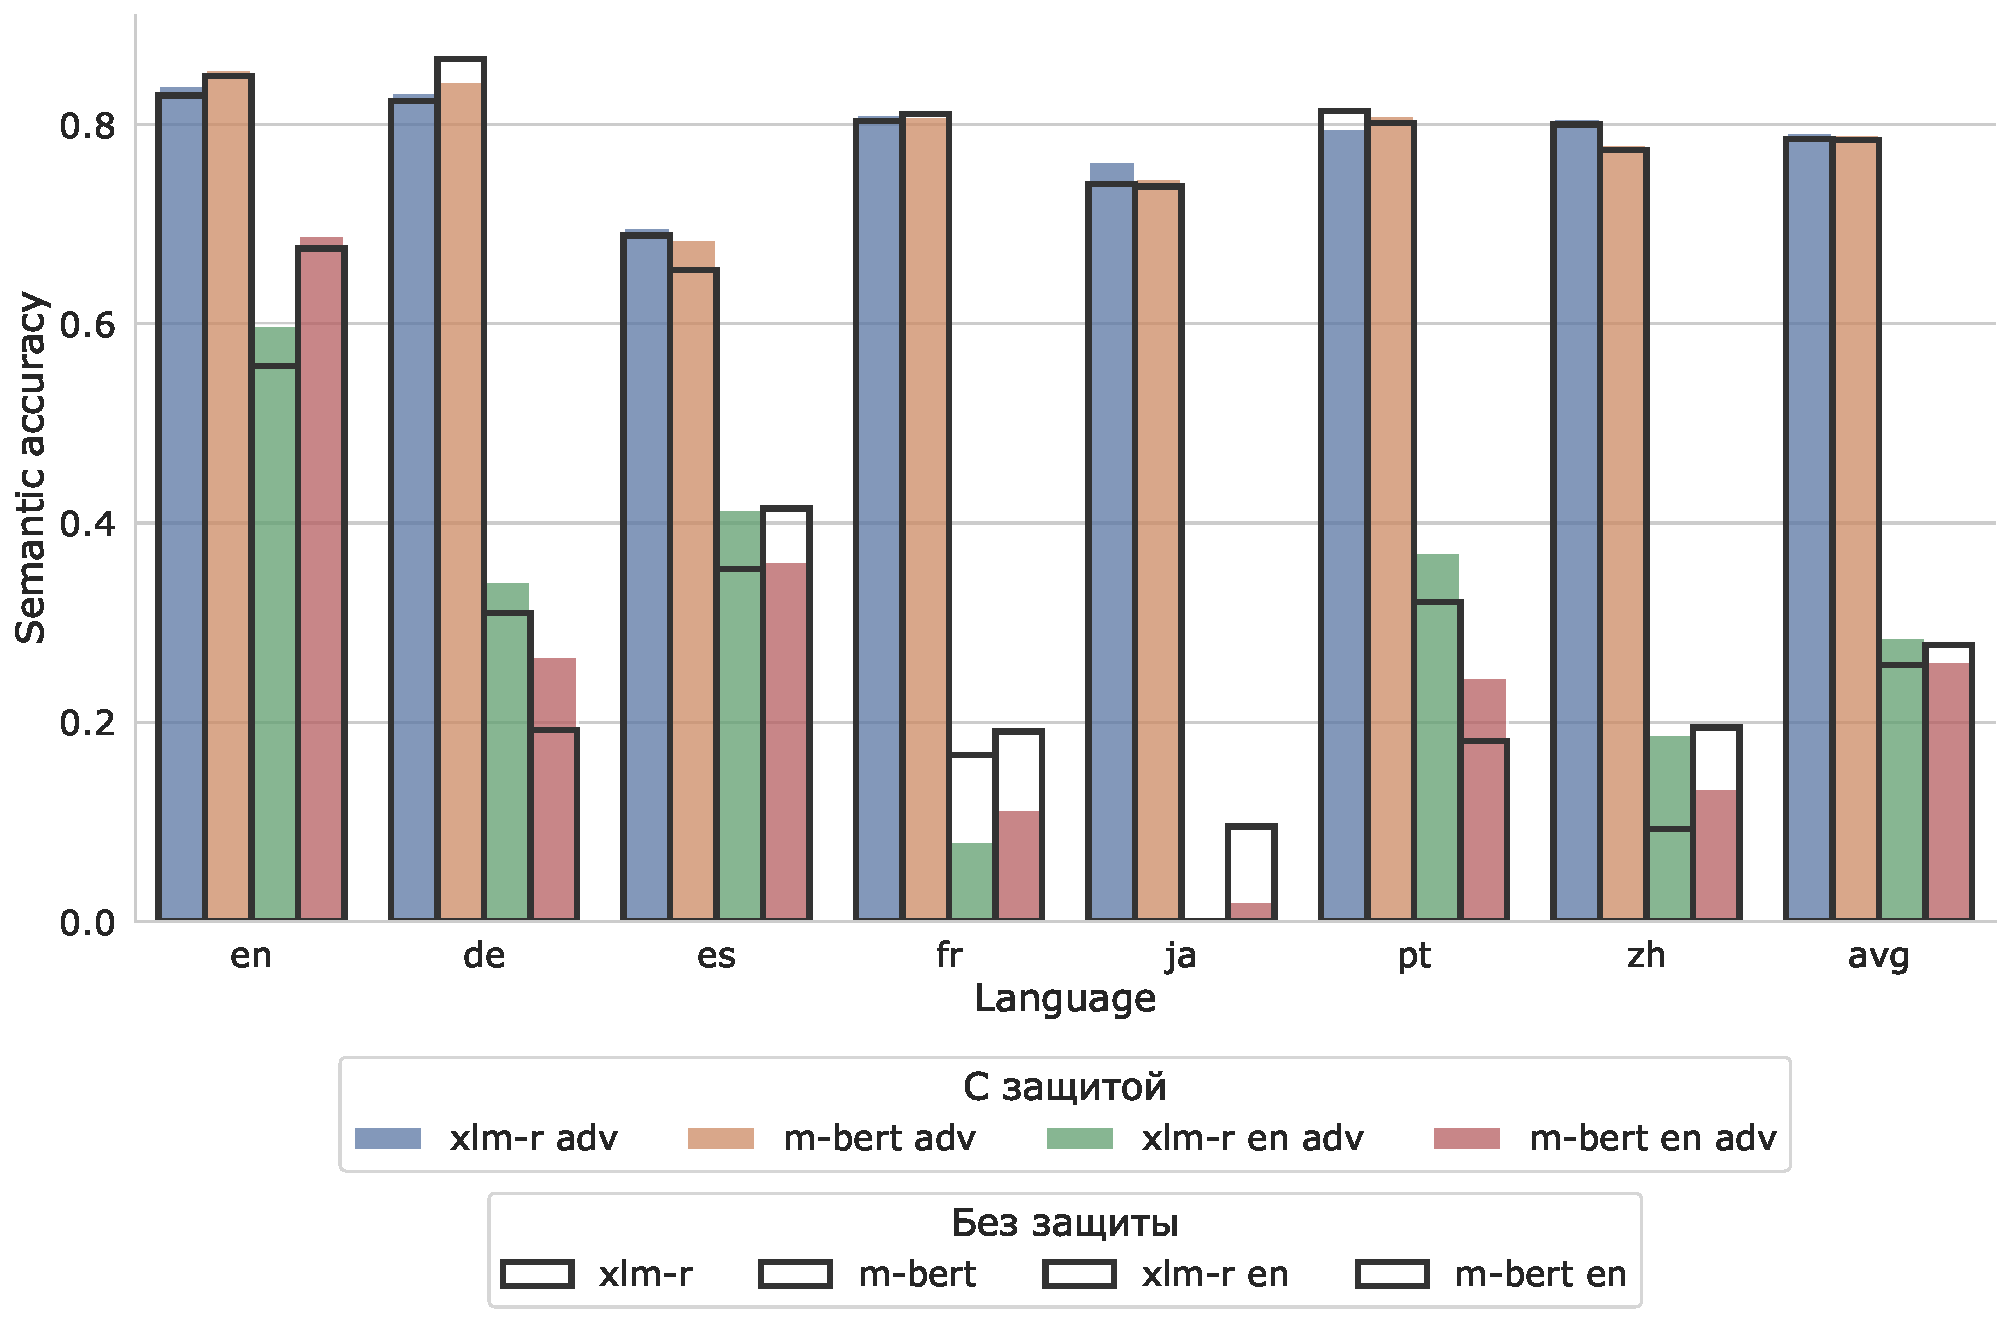
\includegraphics[width=\textwidth]{images/11}
    \caption{Сравнение моделей \textbf{с защитой} между собой \textbf{на тестовой выборке} датасета MultiAtis++ по метрике \textbf{Semantic accuracy}.}\label{fig:figure11}
\end{figure}

\begin{figure}[H]
    \centering
    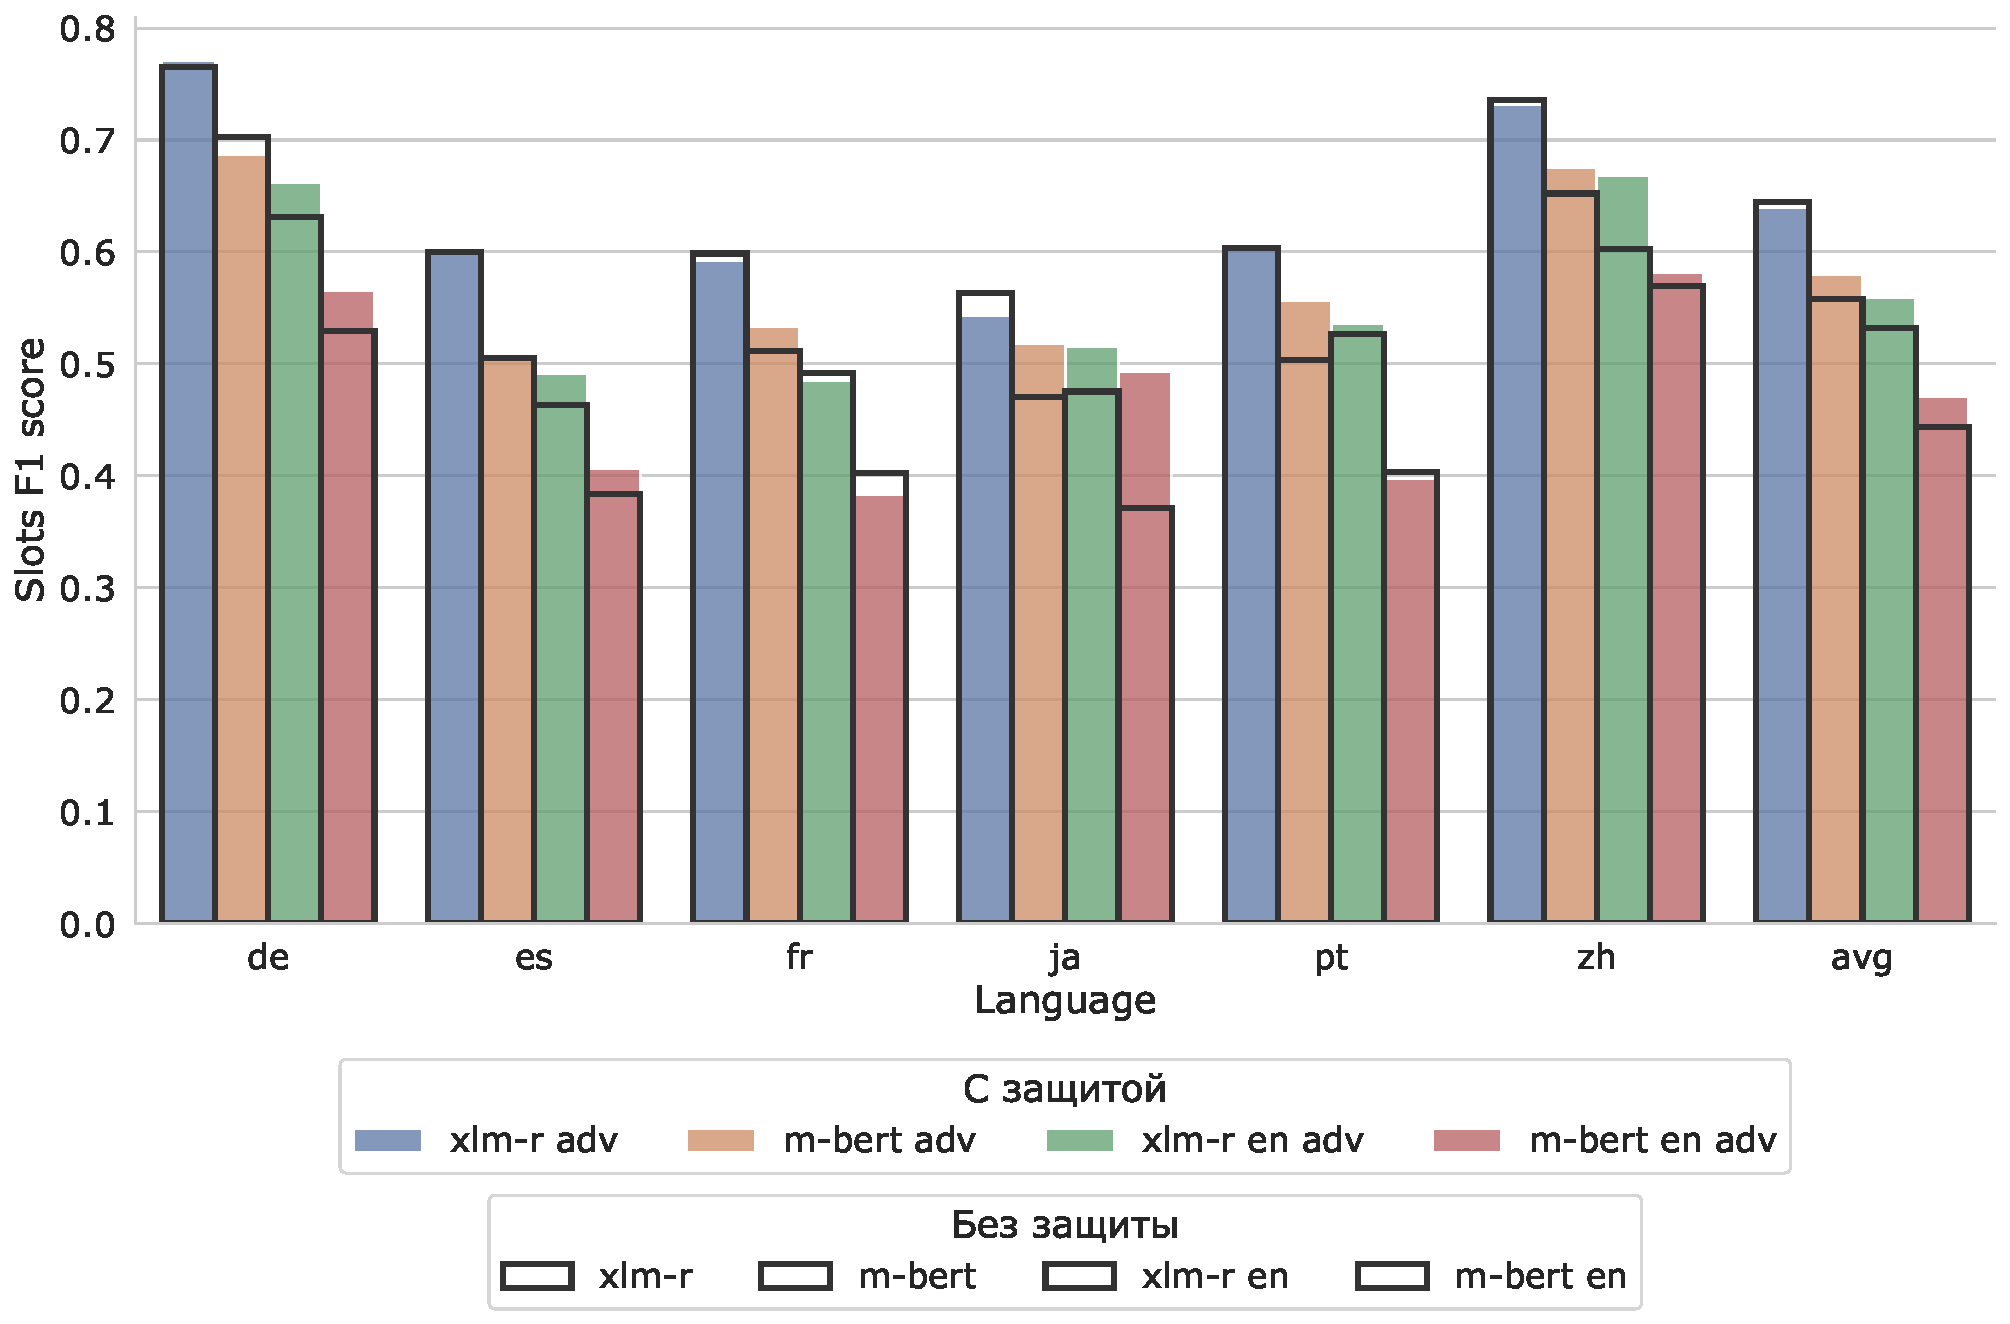
\includegraphics[width=\textwidth]{images/13}
    \caption{Сравнение моделей \textbf{с защитой} между собой после \textbf{word-level} атаки на тестовую выборку датасета MultiAtis++ по метрике \textbf{Slots F1 score}.}\label{fig:figure13}
\end{figure}
\begin{figure}[H]
    \centering
    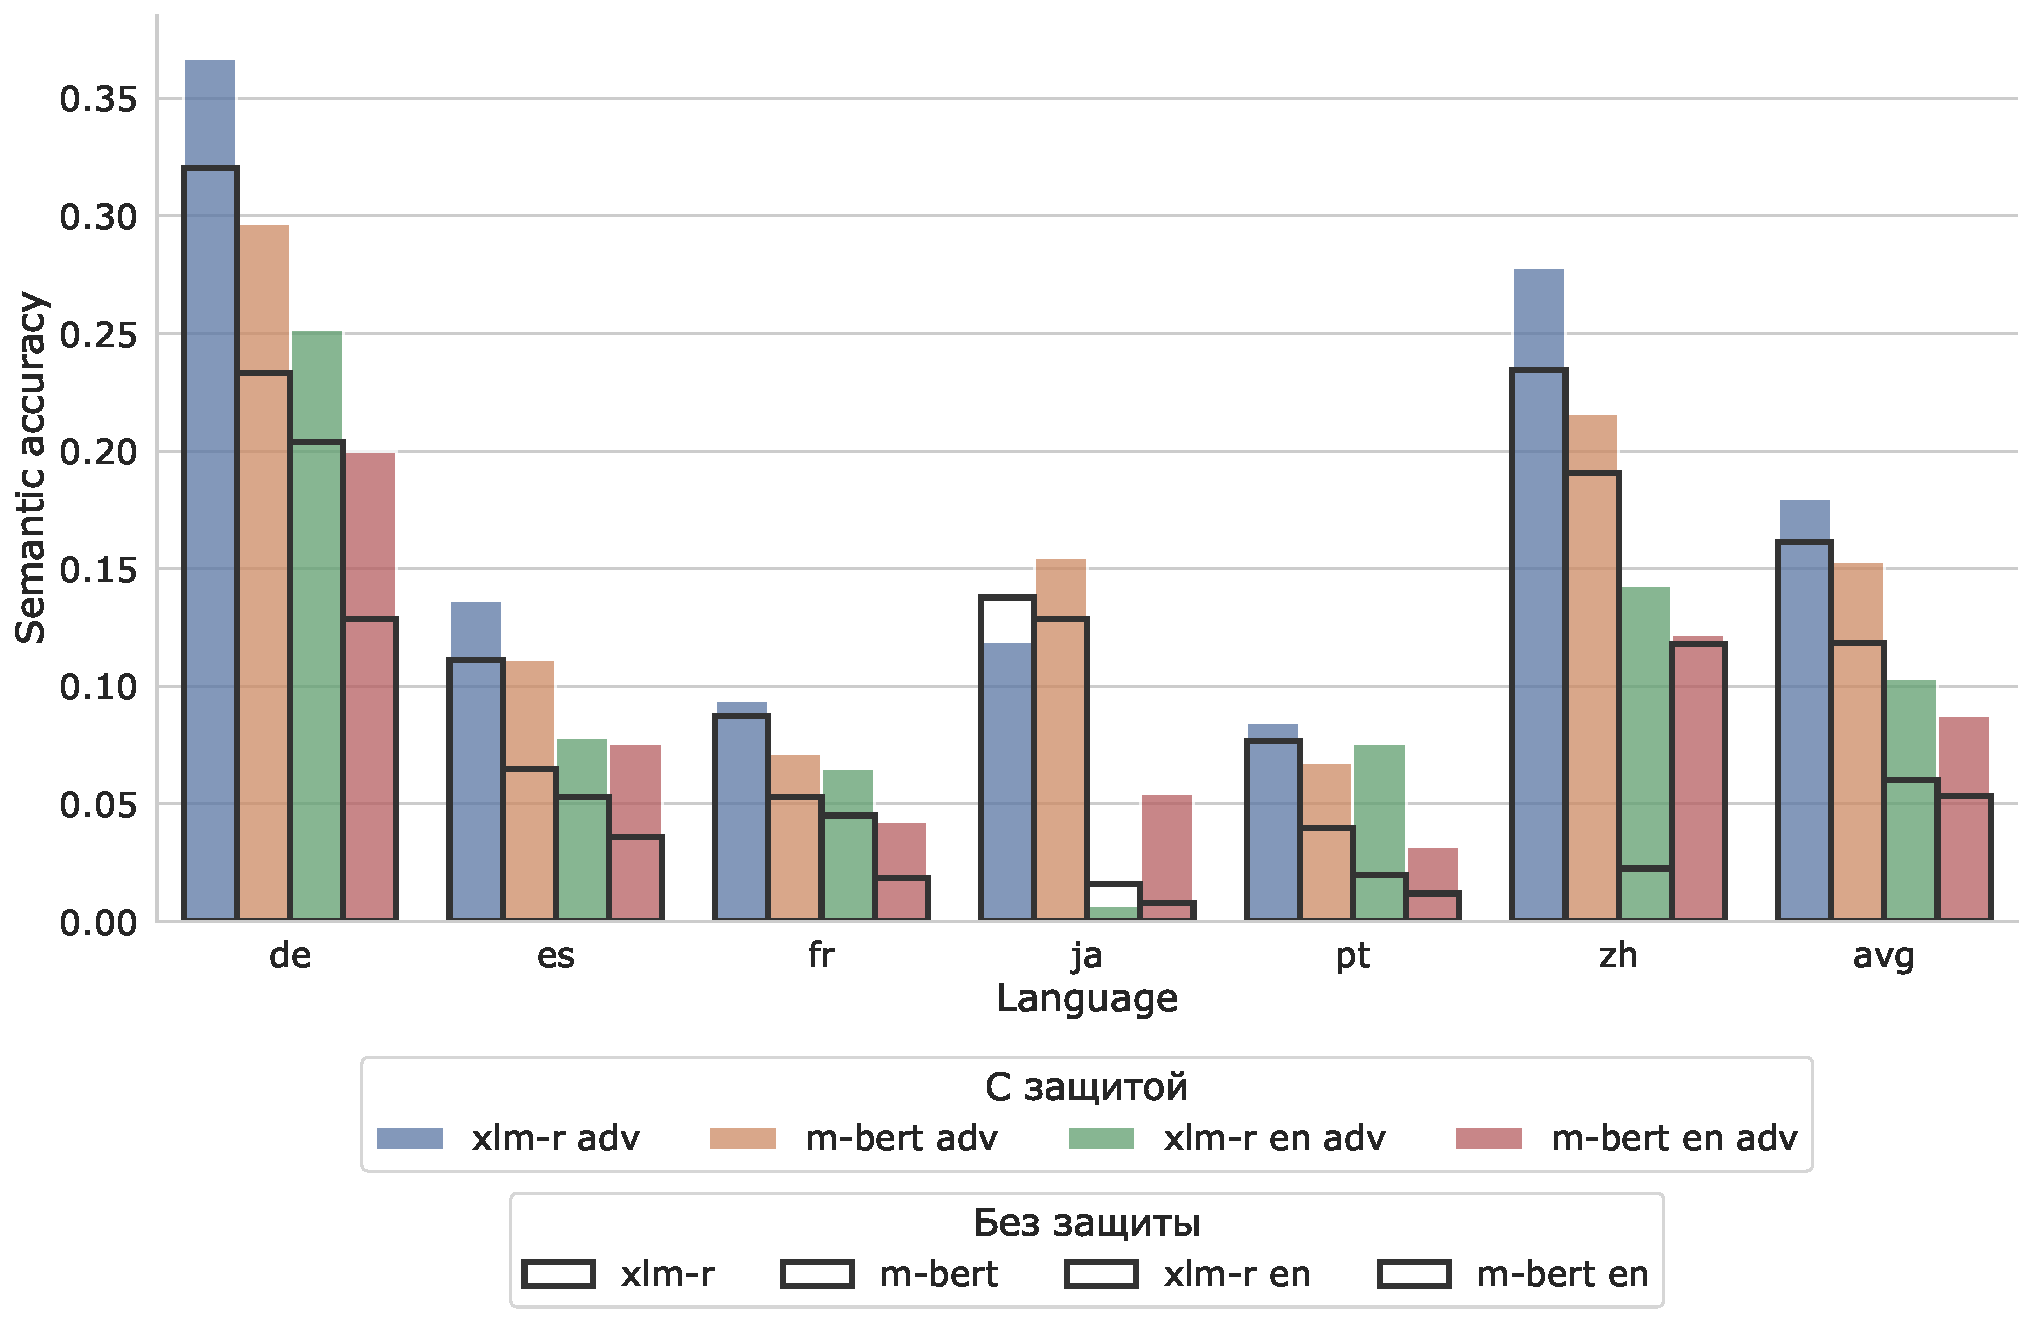
\includegraphics[width=\textwidth]{images/14}
    \caption{Сравнение моделей \textbf{с защитой} между собой после \textbf{word-level} атаки на тестовую выборку датасета MultiAtis++ по метрике \textbf{Semantic accuracy}.}\label{fig:figure14}
\end{figure}

\begin{figure}[H]
    \centering
    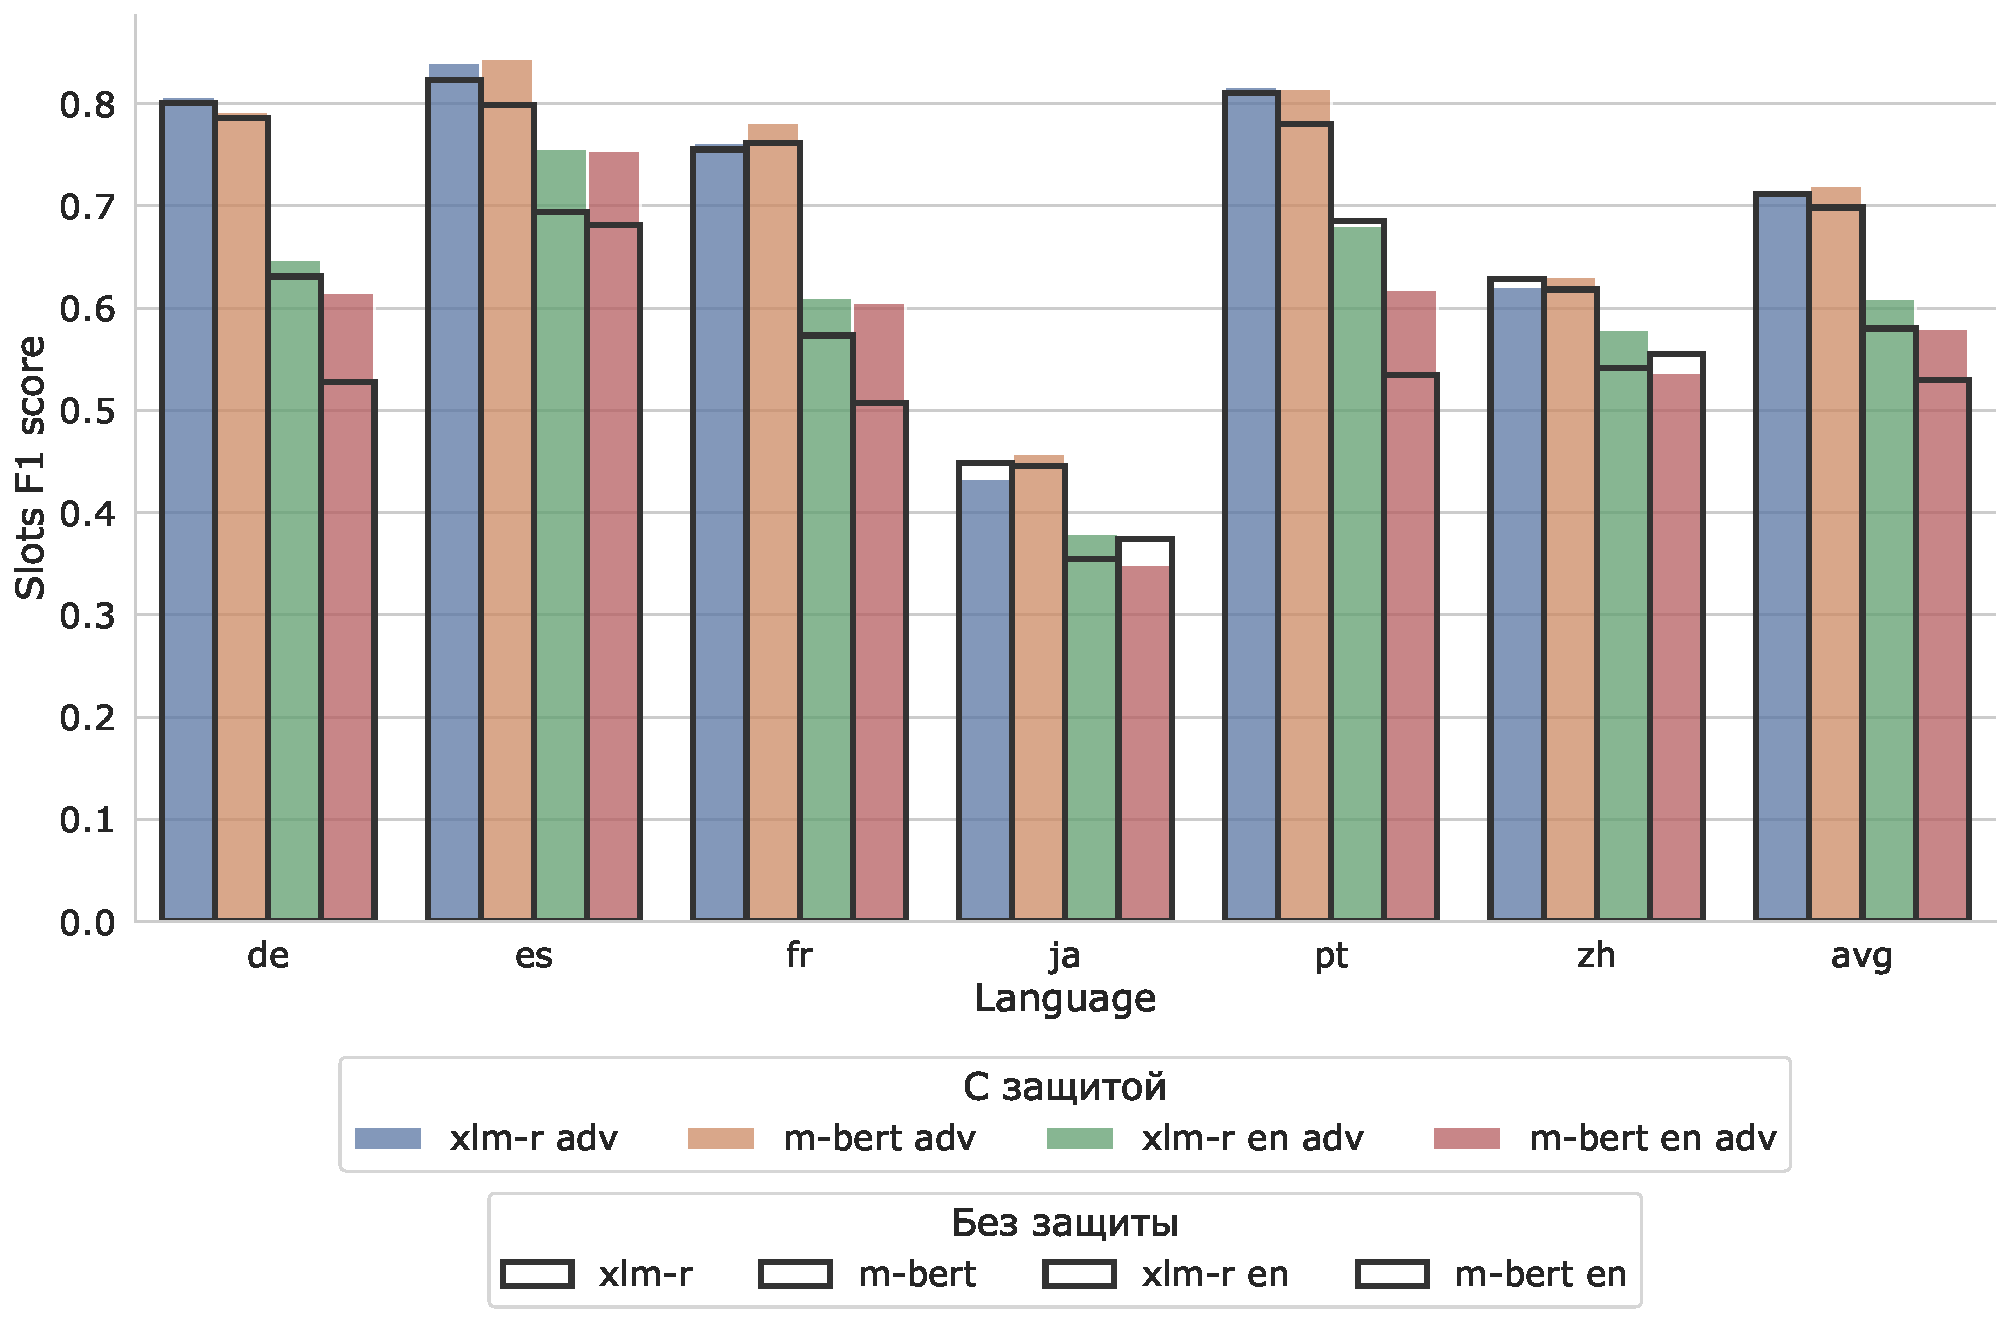
\includegraphics[width=\textwidth]{images/16}
    \caption{Сравнение моделей \textbf{с защитой} между собой после \textbf{phrase-level} атаки на тестовую выборку датасета MultiAtis++ по метрике \textbf{Slots F1 score}.}\label{fig:figure16}
\end{figure}
\begin{figure}[H]
    \centering
    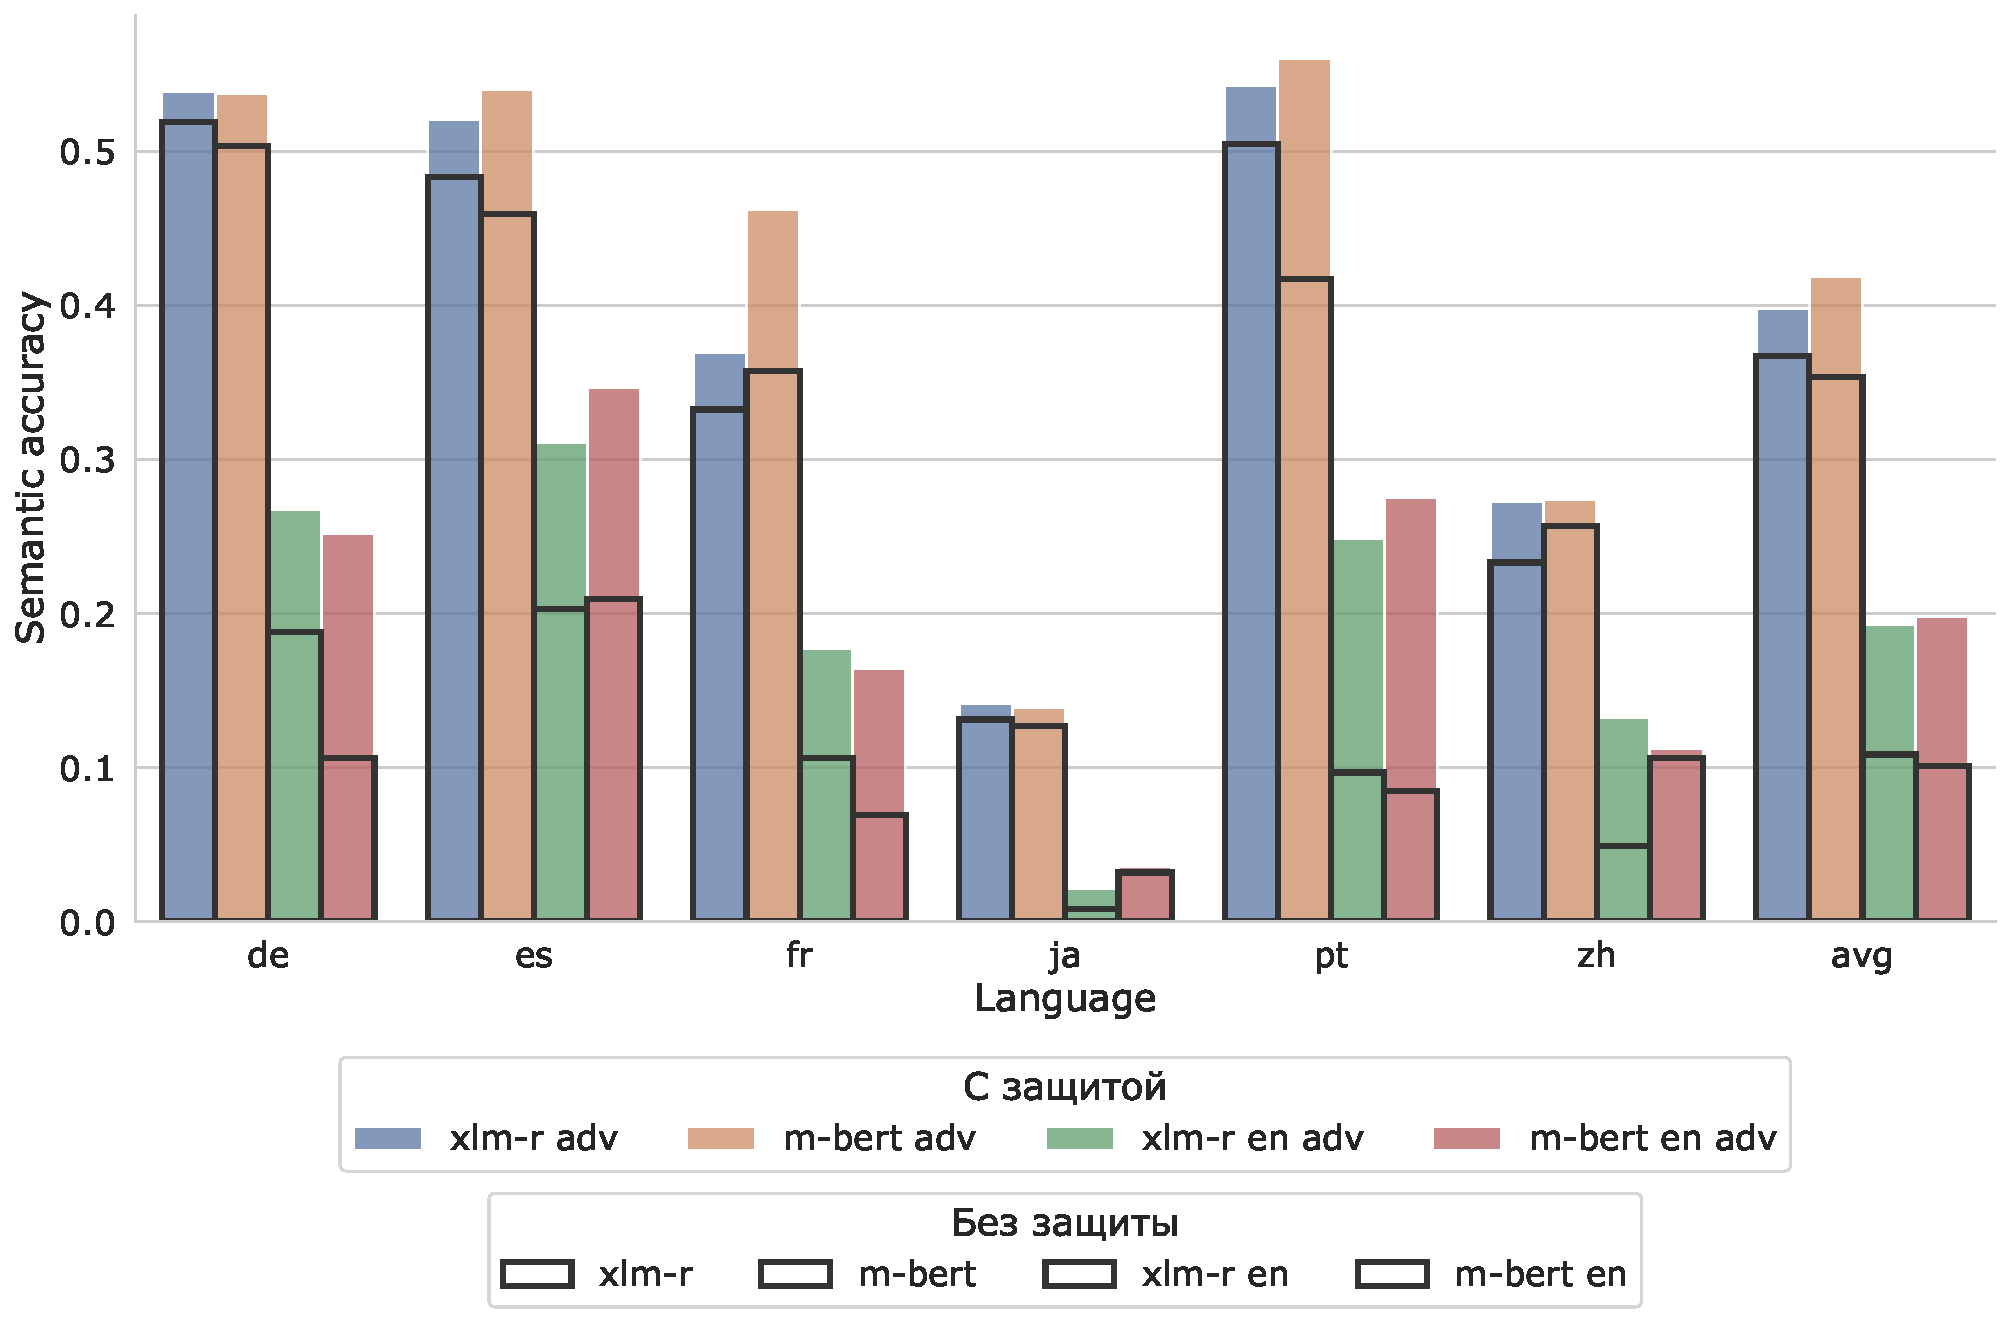
\includegraphics[width=\textwidth]{images/17}
    \caption{Сравнение моделей \textbf{с защитой} между собой после \textbf{phrase-level} атаки на тестовую выборку датасета MultiAtis++ по метрике \textbf{Semantic accuracy}.}\label{fig:figure17}
\end{figure}

\newpage

\subsection{Таблицы с результатами экспериментов}\label{subsec:tables}

\begin{table}[H]
	\resizebox{\textwidth}{!}{
		\begin{tabular}{|>{\bfseries}l|c|c|c|c|c|c|c|c|}
			\hline
			& en & de & es & fr & ja & pt & zh & avg \\ \hline
			xlm-r&$0.980$ & $0.975$ & $0.968$ & $0.972$ & $0.977$ & $0.970$ & $0.968$ & $0.973$ \\ \hline
			m-bert&$0.977$ & $0.977$ & $0.963$ & $0.966$ & $0.959$ & $0.967$ & $0.962$ & $0.967$ \\ \hline
			xlm-r en&$0.903$ & $0.885$ & $0.882$ & $0.879$ & $0.830$ & $0.846$ & $0.856$ & $0.869$ \\ \hline
			m-bert en&$0.951$ & $0.828$ & $0.865$ & $0.877$ & $0.750$ & $0.853$ & $0.795$ & $0.845$ \\ \hline
		\end{tabular}
	}\caption{Сравнение моделей между собой \textbf{на тестовой выборке} датасета MultiAtis++ по метрике \textbf{Intent accuracy}. По колонкам языки тестовых подвыборок, по рядам тестируемые модели.}\label{tab:table0}
\end{table}
\begin{table}[H]
	\resizebox{\textwidth}{!}{
		\begin{tabular}{|>{\bfseries}l|c|c|c|c|c|c|c|c|}
			\hline
			& en & de & es & fr & ja & pt & zh & avg \\ \hline
			xlm-r&$0.945$ & $0.937$ & $0.902$ & $0.924$ & $0.931$ & $0.927$ & $0.948$ & $0.931$ \\ \hline
			m-bert&$0.947$ & $0.951$ & $0.895$ & $0.931$ & $0.933$ & $0.924$ & $0.944$ & $0.932$ \\ \hline
			xlm-r en&$0.871$ & $0.702$ & $0.750$ & $0.629$ & $0.535$ & $0.715$ & $0.707$ & $0.701$ \\ \hline
			m-bert en&$0.902$ & $0.553$ & $0.787$ & $0.524$ & $0.643$ & $0.517$ & $0.678$ & $0.658$ \\ \hline
		\end{tabular}
	}\caption{Сравнение моделей между собой \textbf{на тестовой выборке} датасета MultiAtis++ по метрике \textbf{Slots F1 score}. По колонкам языки тестовых подвыборок, по рядам тестируемые модели.}\label{tab:table1}
\end{table}
\begin{table}[H]
	\resizebox{\textwidth}{!}{
		\begin{tabular}{|>{\bfseries}l|c|c|c|c|c|c|c|c|}
			\hline
			& en & de & es & fr & ja & pt & zh & avg \\ \hline
			xlm-r&$0.829$ & $0.824$ & $0.689$ & $0.804$ & $0.740$ & $0.813$ & $0.800$ & $0.786$ \\ \hline
			m-bert&$0.849$ & $0.866$ & $0.654$ & $0.811$ & $0.738$ & $0.801$ & $0.775$ & $0.785$ \\ \hline
			xlm-r en&$0.558$ & $0.310$ & $0.354$ & $0.167$ & $0.000$ & $0.321$ & $0.093$ & $0.257$ \\ \hline
			m-bert en&$0.675$ & $0.192$ & $0.415$ & $0.191$ & $0.095$ & $0.181$ & $0.195$ & $0.278$ \\ \hline
		\end{tabular}
	}\caption{Сравнение моделей между собой \textbf{на тестовой выборке} датасета MultiAtis++ по метрике \textbf{Semantic accuracy}. По колонкам языки тестовых подвыборок, по рядам тестируемые модели.}\label{tab:table2}
\end{table}

\begin{table}[H]
	\resizebox{\textwidth}{!}{
		\begin{tabular}{|>{\bfseries}l|c|c|c|c|c|c|c|}
			\hline
			& de & es & fr & ja & pt & zh & avg \\ \hline
			xlm-r&$0.934$ & $0.881$ & $0.866$ & $0.842$ & $0.894$ & $0.890$ & $0.885$ \\ \hline
			m-bert&$0.902$ & $0.881$ & $0.858$ & $0.868$ & $0.854$ & $0.865$ & $0.871$ \\ \hline
			xlm-r en&$0.862$ & $0.804$ & $0.768$ & $0.731$ & $0.572$ & $0.828$ & $0.761$ \\ \hline
			m-bert en&$0.812$ & $0.758$ & $0.793$ & $0.760$ & $0.755$ & $0.780$ & $0.776$ \\ \hline
		\end{tabular}
	}\caption{Сравнение моделей между собой после \textbf{word-level} атаки на тестовую выборку датасета MultiAtis++ по метрике \textbf{Intent accuracy}. По колонкам встраиваемые языки, по рядам тестируемые модели.}\label{tab:table3}
\end{table}
\begin{table}[H]
	\resizebox{\textwidth}{!}{
		\begin{tabular}{|>{\bfseries}l|c|c|c|c|c|c|c|}
			\hline
			& de & es & fr & ja & pt & zh & avg \\ \hline
			xlm-r&$0.765$ & $0.600$ & $0.599$ & $0.564$ & $0.604$ & $0.736$ & $0.645$ \\ \hline
			m-bert&$0.702$ & $0.505$ & $0.511$ & $0.471$ & $0.504$ & $0.652$ & $0.558$ \\ \hline
			xlm-r en&$0.631$ & $0.463$ & $0.492$ & $0.475$ & $0.526$ & $0.603$ & $0.532$ \\ \hline
			m-bert en&$0.529$ & $0.384$ & $0.403$ & $0.371$ & $0.404$ & $0.570$ & $0.443$ \\ \hline
		\end{tabular}
	}\caption{Сравнение моделей между собой после \textbf{word-level} атаки на тестовую выборку датасета MultiAtis++ по метрике \textbf{Slots F1 score}. По колонкам встраиваемые языки, по рядам тестируемые модели.}\label{tab:table4}
\end{table}
\begin{table}[H]
	\resizebox{\textwidth}{!}{
		\begin{tabular}{|>{\bfseries}l|c|c|c|c|c|c|c|}
			\hline
			& de & es & fr & ja & pt & zh & avg \\ \hline
			xlm-r&$0.321$ & $0.111$ & $0.087$ & $0.138$ & $0.077$ & $0.234$ & $0.161$ \\ \hline
			m-bert&$0.233$ & $0.065$ & $0.053$ & $0.128$ & $0.040$ & $0.191$ & $0.118$ \\ \hline
			xlm-r en&$0.204$ & $0.053$ & $0.045$ & $0.016$ & $0.020$ & $0.023$ & $0.060$ \\ \hline
			m-bert en&$0.128$ & $0.036$ & $0.019$ & $0.008$ & $0.012$ & $0.118$ & $0.053$ \\ \hline
		\end{tabular}
	}\caption{Сравнение моделей между собой после \textbf{word-level} атаки на тестовую выборку датасета MultiAtis++ по метрике \textbf{Semantic accuracy}. По колонкам встраиваемые языки, по рядам тестируемые модели.}\label{tab:table5}
\end{table}

\begin{table}[H]
	\resizebox{\textwidth}{!}{
		\begin{tabular}{|>{\bfseries}l|c|c|c|c|c|c|c|}
			\hline
			& de & es & fr & ja & pt & zh & avg \\ \hline
			xlm-r&$0.956$ & $0.950$ & $0.931$ & $0.964$ & $0.955$ & $0.954$ & $0.952$ \\ \hline
			m-bert&$0.943$ & $0.947$ & $0.939$ & $0.943$ & $0.952$ & $0.934$ & $0.943$ \\ \hline
			xlm-r en&$0.850$ & $0.849$ & $0.762$ & $0.799$ & $0.477$ & $0.868$ & $0.767$ \\ \hline
			m-bert en&$0.809$ & $0.845$ & $0.844$ & $0.803$ & $0.864$ & $0.819$ & $0.830$ \\ \hline
		\end{tabular}
	}\caption{Сравнение моделей между собой после \textbf{phrase-level} атаки на тестовую выборку датасета MultiAtis++ по метрике \textbf{Intent accuracy}. По колонкам встраиваемые языки, по рядам тестируемые модели.}\label{tab:table6}
\end{table}
\begin{table}[H]
	\resizebox{\textwidth}{!}{
		\begin{tabular}{|>{\bfseries}l|c|c|c|c|c|c|c|}
			\hline
			& de & es & fr & ja & pt & zh & avg \\ \hline
			xlm-r&$0.801$ & $0.823$ & $0.755$ & $0.449$ & $0.810$ & $0.629$ & $0.711$ \\ \hline
			m-bert&$0.786$ & $0.799$ & $0.761$ & $0.446$ & $0.780$ & $0.618$ & $0.698$ \\ \hline
			xlm-r en&$0.631$ & $0.694$ & $0.573$ & $0.355$ & $0.686$ & $0.541$ & $0.580$ \\ \hline
			m-bert en&$0.528$ & $0.681$ & $0.507$ & $0.374$ & $0.534$ & $0.555$ & $0.530$ \\ \hline
		\end{tabular}
	}\caption{Сравнение моделей между собой после \textbf{phrase-level} атаки на тестовую выборку датасета MultiAtis++ по метрике \textbf{Slots F1 score}. По колонкам встраиваемые языки, по рядам тестируемые модели.}\label{tab:table7}
\end{table}
\begin{table}[H]
	\resizebox{\textwidth}{!}{
		\begin{tabular}{|>{\bfseries}l|c|c|c|c|c|c|c|}
			\hline
			& de & es & fr & ja & pt & zh & avg \\ \hline
			xlm-r&$0.519$ & $0.483$ & $0.332$ & $0.131$ & $0.505$ & $0.233$ & $0.367$ \\ \hline
			m-bert&$0.503$ & $0.460$ & $0.358$ & $0.127$ & $0.417$ & $0.257$ & $0.354$ \\ \hline
			xlm-r en&$0.188$ & $0.203$ & $0.106$ & $0.008$ & $0.097$ & $0.049$ & $0.108$ \\ \hline
			m-bert en&$0.106$ & $0.209$ & $0.069$ & $0.032$ & $0.085$ & $0.106$ & $0.101$ \\ \hline
		\end{tabular}
	}\caption{Сравнение моделей между собой после \textbf{phrase-level} атаки на тестовую выборку датасета MultiAtis++ по метрике \textbf{Semantic accuracy}. По колонкам встраиваемые языки, по рядам тестируемые модели.}\label{tab:table8}
\end{table}

\begin{table}[H]
	\resizebox{\textwidth}{!}{
		\begin{tabular}{|>{\bfseries}l|c|c|c|c|c|c|c|c|}
			\hline
			& en & de & es & fr & ja & pt & zh & avg \\ \hline
			xlm-r adv&$0.976$ & $0.975$ & $0.962$ & $0.975$ & $0.976$ & $0.964$ & $0.968$ & $0.971$ \\ \hline
			m-bert adv&$0.981$ & $0.975$ & $0.960$ & $0.971$ & $0.970$ & $0.971$ & $0.958$ & $0.969$ \\ \hline
			xlm-r en adv&$0.951$ & $0.898$ & $0.895$ & $0.878$ & $0.837$ & $0.907$ & $0.838$ & $0.886$ \\ \hline
			m-bert en adv&$0.958$ & $0.838$ & $0.889$ & $0.864$ & $0.706$ & $0.882$ & $0.748$ & $0.841$ \\ \hline
		\end{tabular}
	}\caption{Сравнение моделей \textbf{с защитой} между собой \textbf{на тестовой выборке} датасета MultiAtis++ по метрике \textbf{Intent accuracy}. По колонкам языки тестовых подвыборок, по рядам тестируемые модели.}\label{tab:table9}
\end{table}
\begin{table}[H]
	\resizebox{\textwidth}{!}{
		\begin{tabular}{|>{\bfseries}l|c|c|c|c|c|c|c|c|}
			\hline
			& en & de & es & fr & ja & pt & zh & avg \\ \hline
			xlm-r adv&$0.948$ & $0.942$ & $0.906$ & $0.927$ & $0.933$ & $0.924$ & $0.950$ & $0.933$ \\ \hline
			m-bert adv&$0.952$ & $0.942$ & $0.903$ & $0.932$ & $0.934$ & $0.925$ & $0.945$ & $0.933$ \\ \hline
			xlm-r en adv&$0.880$ & $0.711$ & $0.780$ & $0.583$ & $0.534$ & $0.705$ & $0.746$ & $0.705$ \\ \hline
			m-bert en adv&$0.907$ & $0.613$ & $0.756$ & $0.522$ & $0.456$ & $0.553$ & $0.605$ & $0.630$ \\ \hline
		\end{tabular}
	}\caption{Сравнение моделей \textbf{с защитой} между собой \textbf{на тестовой выборке} датасета MultiAtis++ по метрике \textbf{Slots F1 score}. По колонкам языки тестовых подвыборок, по рядам тестируемые модели.}\label{tab:table10}
\end{table}
\begin{table}[H]
	\resizebox{\textwidth}{!}{
		\begin{tabular}{|>{\bfseries}l|c|c|c|c|c|c|c|c|}
			\hline
			& en & de & es & fr & ja & pt & zh & avg \\ \hline
			xlm-r adv&$0.840$ & $0.832$ & $0.697$ & $0.811$ & $0.763$ & $0.796$ & $0.807$ & $0.792$ \\ \hline
			m-bert adv&$0.856$ & $0.844$ & $0.685$ & $0.808$ & $0.746$ & $0.809$ & $0.780$ & $0.790$ \\ \hline
			xlm-r en adv&$0.599$ & $0.342$ & $0.413$ & $0.081$ & $0.001$ & $0.371$ & $0.188$ & $0.285$ \\ \hline
			m-bert en adv&$0.689$ & $0.266$ & $0.362$ & $0.113$ & $0.020$ & $0.245$ & $0.134$ & $0.261$ \\ \hline
		\end{tabular}
	}\caption{Сравнение моделей \textbf{с защитой} между собой \textbf{на тестовой выборке} датасета MultiAtis++ по метрике \textbf{Semantic accuracy}. По колонкам языки тестовых подвыборок, по рядам тестируемые модели.}\label{tab:table11}
\end{table}

\begin{table}[H]
	\resizebox{\textwidth}{!}{
		\begin{tabular}{|>{\bfseries}l|c|c|c|c|c|c|c|}
			\hline
			& de & es & fr & ja & pt & zh & avg \\ \hline
			xlm-r adv&$0.930$ & $0.907$ & $0.883$ & $0.833$ & $0.911$ & $0.869$ & $0.889$ \\ \hline
			m-bert adv&$0.919$ & $0.913$ & $0.883$ & $0.881$ & $0.902$ & $0.848$ & $0.891$ \\ \hline
			xlm-r en adv&$0.874$ & $0.813$ & $0.830$ & $0.793$ & $0.834$ & $0.796$ & $0.824$ \\ \hline
			m-bert en adv&$0.852$ & $0.824$ & $0.805$ & $0.710$ & $0.857$ & $0.779$ & $0.804$ \\ \hline
		\end{tabular}
	}\caption{Сравнение моделей \textbf{с защитой} между собой после \textbf{word-level} атаки на тестовую выборку датасета MultiAtis++ по метрике \textbf{Intent accuracy}. По колонкам встраиваемые языки, по рядам тестируемые модели.}\label{tab:table12}
\end{table}
\begin{table}[H]
	\resizebox{\textwidth}{!}{
		\begin{tabular}{|>{\bfseries}l|c|c|c|c|c|c|c|}
			\hline
			& de & es & fr & ja & pt & zh & avg \\ \hline
			xlm-r adv&$0.771$ & $0.598$ & $0.592$ & $0.543$ & $0.604$ & $0.731$ & $0.640$ \\ \hline
			m-bert adv&$0.687$ & $0.507$ & $0.533$ & $0.518$ & $0.557$ & $0.675$ & $0.580$ \\ \hline
			xlm-r en adv&$0.662$ & $0.491$ & $0.485$ & $0.516$ & $0.536$ & $0.668$ & $0.560$ \\ \hline
			m-bert en adv&$0.565$ & $0.407$ & $0.384$ & $0.493$ & $0.398$ & $0.582$ & $0.471$ \\ \hline
		\end{tabular}
	}\caption{Сравнение моделей \textbf{с защитой} между собой после \textbf{word-level} атаки на тестовую выборку датасета MultiAtis++ по метрике \textbf{Slots F1 score}. По колонкам встраиваемые языки, по рядам тестируемые модели.}\label{tab:table13}
\end{table}
\begin{table}[H]
	\resizebox{\textwidth}{!}{
		\begin{tabular}{|>{\bfseries}l|c|c|c|c|c|c|c|}
			\hline
			& de & es & fr & ja & pt & zh & avg \\ \hline
			xlm-r adv&$0.367$ & $0.136$ & $0.094$ & $0.119$ & $0.085$ & $0.278$ & $0.180$ \\ \hline
			m-bert adv&$0.297$ & $0.111$ & $0.072$ & $0.155$ & $0.068$ & $0.216$ & $0.153$ \\ \hline
			xlm-r en adv&$0.252$ & $0.078$ & $0.065$ & $0.007$ & $0.075$ & $0.143$ & $0.103$ \\ \hline
			m-bert en adv&$0.200$ & $0.075$ & $0.042$ & $0.054$ & $0.032$ & $0.122$ & $0.088$ \\ \hline
		\end{tabular}
	}\caption{Сравнение моделей \textbf{с защитой} между собой после \textbf{word-level} атаки на тестовую выборку датасета MultiAtis++ по метрике \textbf{Semantic accuracy}. По колонкам встраиваемые языки, по рядам тестируемые модели.}\label{tab:table14}
\end{table}

\begin{table}[H]
	\resizebox{\textwidth}{!}{
		\begin{tabular}{|>{\bfseries}l|c|c|c|c|c|c|c|}
			\hline
			& de & es & fr & ja & pt & zh & avg \\ \hline
			xlm-r adv&$0.951$ & $0.944$ & $0.927$ & $0.962$ & $0.958$ & $0.951$ & $0.949$ \\ \hline
			m-bert adv&$0.960$ & $0.956$ & $0.948$ & $0.951$ & $0.956$ & $0.954$ & $0.954$ \\ \hline
			xlm-r en adv&$0.873$ & $0.854$ & $0.878$ & $0.829$ & $0.865$ & $0.837$ & $0.856$ \\ \hline
			m-bert en adv&$0.838$ & $0.869$ & $0.846$ & $0.755$ & $0.906$ & $0.774$ & $0.831$ \\ \hline
		\end{tabular}
	}\caption{Сравнение моделей \textbf{с защитой} между собой после \textbf{phrase-level} атаки на тестовую выборку датасета MultiAtis++ по метрике \textbf{Intent accuracy}. По колонкам встраиваемые языки, по рядам тестируемые модели.}\label{tab:table15}
\end{table}
\begin{table}[H]
	\resizebox{\textwidth}{!}{
		\begin{tabular}{|>{\bfseries}l|c|c|c|c|c|c|c|}
			\hline
			& de & es & fr & ja & pt & zh & avg \\ \hline
			xlm-r adv&$0.808$ & $0.840$ & $0.762$ & $0.433$ & $0.817$ & $0.621$ & $0.713$ \\ \hline
			m-bert adv&$0.793$ & $0.844$ & $0.782$ & $0.458$ & $0.815$ & $0.631$ & $0.720$ \\ \hline
			xlm-r en adv&$0.648$ & $0.756$ & $0.610$ & $0.380$ & $0.681$ & $0.580$ & $0.609$ \\ \hline
			m-bert en adv&$0.615$ & $0.754$ & $0.606$ & $0.350$ & $0.618$ & $0.537$ & $0.580$ \\ \hline
		\end{tabular}
	}\caption{Сравнение моделей \textbf{с защитой} между собой после \textbf{phrase-level} атаки на тестовую выборку датасета MultiAtis++ по метрике \textbf{Slots F1 score}. По колонкам встраиваемые языки, по рядам тестируемые модели.}\label{tab:table16}
\end{table}
\begin{table}[H]
	\resizebox{\textwidth}{!}{
		\begin{tabular}{|>{\bfseries}l|c|c|c|c|c|c|c|}
			\hline
			& de & es & fr & ja & pt & zh & avg \\ \hline
			xlm-r adv&$0.539$ & $0.521$ & $0.370$ & $0.142$ & $0.543$ & $0.273$ & $0.398$ \\ \hline
			m-bert adv&$0.538$ & $0.540$ & $0.462$ & $0.139$ & $0.560$ & $0.274$ & $0.419$ \\ \hline
			xlm-r en adv&$0.268$ & $0.311$ & $0.177$ & $0.021$ & $0.249$ & $0.132$ & $0.193$ \\ \hline
			m-bert en adv&$0.252$ & $0.347$ & $0.164$ & $0.036$ & $0.275$ & $0.113$ & $0.198$ \\ \hline
		\end{tabular}
	}\caption{Сравнение моделей \textbf{с защитой} между собой после \textbf{phrase-level} атаки на тестовую выборку датасета MultiAtis++ по метрике \textbf{Semantic accuracy}. По колонкам встраиваемые языки, по рядам тестируемые модели.}\label{tab:table17}
\end{table}

